%%%%%%%%%%%%%%%%%%%%%%%%%%%%%%%%%%%%%%%%%%%%%%%%%%%%%%%%%%%%%%%%%%%%%%%%%%%%%%%%
%2345678901234567890123456789012345678901234567890123456789012345678901234567890
%        1         2         3         4         5         6         7         8

\documentclass[letterpaper, 10 pt, conference]{ieeeconf}  % Comment this line out if you need a4paper

%\documentclass[a4paper, 10pt, conference]{ieeeconf}      % Use this line for a4 paper

\IEEEoverridecommandlockouts                              % This command is only needed if 
                                                          % you want to use the \thanks command

\overrideIEEEmargins                                      % Needed to meet printer requirements.

%In case you encounter the following error:
%Error 1010 The PDF file may be corrupt (unable to open PDF file) OR
%Error 1000 An error occurred while parsing a contents stream. Unable to analyze the PDF file.
%This is a known problem with pdfLaTeX conversion filter. The file cannot be opened with acrobat reader
%Please use one of the alternatives below to circumvent this error by uncommenting one or the other
%\pdfobjcompresslevel=0
%\pdfminorversion=4

% See the \addtolength command later in the file to balance the column lengths
% on the last page of the document

% The following packages can be found on http:\\www.ctan.org
% \usepackage{graphics} % for pdf, bitmapped graphics files
\usepackage{epsfig} % for postscript graphics files
%\usepackage{mathptmx} % assumes new font selection scheme installed
%\usepackage{times} % assumes new font selection scheme installed
\usepackage{amsmath} % assumes amsmath package installed
\usepackage{amssymb}  % assumes amsmath package installed
\usepackage{multirow}

%%%%%%%%%% my packages%%%%%%%%%%%%%%%%%
\usepackage{hyperref}       % hyperlinks
\usepackage{url}            % simple URL typesetting
\usepackage{booktabs}       % professional-quality tables

\usepackage{nicefrac}       % compact symbols for 1/2, etc.
\usepackage{microtype}      % microtypography
\usepackage{xcolor}         % colors


\usepackage[scientific-notation=true]{siunitx}


\usepackage{microtype}
\usepackage{graphicx}
% \usepackage{subfigure}
% \usepackage{subfig}
% \usepackage{subcaption}
% \usepackage{cleveref}

\usepackage{amsfonts}       % blackboard math symbols
\usepackage{amsmath}
\usepackage{bbm}

% \usepackage{algorithm2e}
\usepackage{algorithm}
\usepackage{algorithmic}

\let\labelindent\relax
\usepackage{enumitem}

\usepackage{soul}

\usepackage{cuted}

\newcommand{\mathcolorbox}[2]{\colorbox{#1}{$\displaystyle #2$}}


% shortcuts
\newcommand{\todo}[1]{\textbf{{\color{red} TODO:} #1}}
\newcommand{\etal}{{\em et al. }}

% math
\newcommand{\cS}{\mathcal{S}}
\newcommand{\cP}{\mathcal{P}}
\newcommand{\cA}{\mathcal{A}}
\newcommand{\cR}{\mathcal{R}}
\newcommand{\cD}{\mathcal{D}}

\newcommand{\cH}{\mathcal{H}} %entropy
\newcommand{\cL}{\mathcal{L}} %loss fct

\newcommand{\stt}{s_t}
\newcommand{\at}{a_t}
\newcommand{\rt}{r_t}
\newcommand{\stone}{s_{t+1}}
\newcommand{\atone}{a_{t+1}}

\newcommand{\sa}{(s, a)}
\newcommand{\stat}{(\st, \at)}
\newcommand{\sttatt}{(\stone, \atone)}

% \newcommand{\E}{\mathbb{E}} % expectation
\DeclareMathOperator*{\E}{\mathbb{E}} % expectation
% \DeclareMathOperator*{\E}{E} % expectation
% \newcommand{\idc}[1]{\mathds{1}\left[#1\right]}  % indicator function
% \newcommand{\idc}[1]{\mathbbm{1}\big[#1\big]}  % indicator function
\newcommand{\idc}[1]{1\big[#1\big]}  % indicator function

% \mathbb{1}

\DeclareMathOperator*{\argmax}{arg\,max}
\DeclareMathOperator*{\argmin}{\arg\,min}

% for this paper
\newcommand{\bmax}{\beta_{max}}
\newcommand{\bmin}{\beta_{min}}

\newcommand{\qhat}{\hat{Q}}
\newcommand{\qhatpi}{\hat{Q}^{\pi}}
\newcommand{\qpi}{Q^{\pi}}
\newcommand{\qbeta}{Q_{\beta}}
\newcommand{\qhatbeta}{\hat{Q}_{\beta}}


% algorithms
\newcommand{\pluseq}{\mathrel{+}=}




\newtheorem{theorem}{Theorem}



\setlength{\skip\footins}{0.6pc plus 5pt minus 2pt}



\title{\LARGE \bf
Adaptively Calibrated Critic Estimates for Deep Reinforcement Learning
}

\author{Nicolai Dorka$^{1}$ and Tim Welschehold$^{1}$ and Joschka Bödecker$^{1}$ and Wolfram Burgard$^{2}$% <-this % stops a space

\thanks{Authors are with: $^{1}$University of Freiburg and $^{2}$ University of Technology Nuremberg, Germany.
        {\tt\small dorka@cs.uni-freiburg.de}.}%
\thanks{This work was supported by the European Union’s Horizon 2020 research and innovation program under grant agreement No 871449-OpenDR.}%
        }


\begin{document}



\maketitle
\thispagestyle{empty}
\pagestyle{empty}


%%%%%%%%%%%%%%%%%%%%%%%%%%%%%%%%%%%%%%%%%%%%%%%%%%%%%%%%%%%%%%%%%%%%%%%%%%%%%%%%
\begin{abstract}

Accurate value estimates are important for off-policy reinforcement learning. 
Algorithms based on temporal difference learning typically are prone to an over- or underestimation bias building up over time.
In this paper, we propose a general method called Adaptively Calibrated Critics (ACC) that uses the most recent high variance but unbiased on-policy rollouts to alleviate the bias of the low variance temporal difference targets.
We apply ACC to Truncated Quantile Critics~\cite{tqc}, which is an algorithm for continuous control that allows regulation of the bias with a hyperparameter tuned per environment.
The resulting algorithm adaptively adjusts the parameter during training rendering hyperparameter search unnecessary 
and sets a new state of the art on the OpenAI gym continuous control benchmark among all algorithms
that do not tune hyperparameters for each environment.
ACC further achieves improved results on different tasks from the Meta-World robot benchmark.
Additionally, we demonstrate the generality of ACC by applying it to TD3~\cite{td3} and showing an improved performance also in this setting. 
\end{abstract}


%%%%%%%%%%%%%%%%%%%%%%%%%%%%%%%%%%%%%%%%%%%%%%%%%%%%%%%%%%%%%%%%%%%%%%%%%%%%%%%%


\section{Introduction}






Off-policy reinforcement learning is an important research direction as the reuse of old experience promises to make these methods more sample efficient than their on-policy counterparts. This is an important property for many applications such as robotics where  interactions with the environment are very time- and cost-intensive.
Many successful off-policy methods make use of a learned Q-value function~\cite{td3,SAC,hessel2018rainbow,dqn15}. 
If the action space is discrete the Q-function can be directly  used to generate actions while for continuous action spaces it is usually used in an actor-critic setting where the policy is trained to choose actions that maximize the Q-function. In both cases accurate estimates of the Q-values are of crucial importance.

% \looseness=-1
% \looseness=-1 \spaceskip= 2pt plus 1pt minus 1.5pt  \spaceskip= 3pt plus 2pt minus 2pt
Unfortunately, learning the Q-function off-policy can lead to an overestimation bias~\cite{Thrun+Schwartz:1993}.
Especially when a nonlinear function approximator is used to model the Q-function, there are many potential sources of bias.
Different heuristics were proposed for their mitigation, such as the double estimator in the case of discrete action spaces~\cite{hasselt2016deepdouble} or taking the minimum of two estimates in the case of continuous actions~\cite{td3}.
While these methods successfully prevent extreme overestimation, due to their coarse nature, they can  still induce under- or overestimation bias to a varying degree depending on the environment~\cite{Lan2020Maxmin}.\looseness=-1

To overcome these problems we propose a principled and general method to alleviate the bias called Adaptively Calibrated Critics (ACC).
Our algorithm uses the most recent on-policy rollouts to determine the current bias of the Q-estimates and adjusts a bias controlling parameter accordingly.
This parameter adapts the size of the temporal difference (TD) targets  such that the bias can be corrected in the subsequent updates.
As the parameter changes slower than the rollout returns, our method still benefits from stable and low-variance temporal difference targets, while it incorporates the information from unbiased but high variance samples from the recent policy to reduce the bias. 


{\spaceskip= 2pt plus 1pt minus 1.5pt  \spaceskip= 3pt plus 2pt minus 2pt We apply ACC to Truncated Quantile Critics (TQC) \cite{tqc}, which is a recent off-policy actor-critic algorithm for continuous control showing strong performance on various tasks. 
In TQC the bias can be controlled in a finegrained way with the help of a hyperparameter that has to be tuned for every environment.
ACC allows to automatically adjusts this parameter online during the training in the environment.
As a result, it eliminates the need to tune this hyperparameter in a new environment, which is very expensive or even infeasible for many applications.}

% \looseness=-1
We evaluate our algorithm on a range of continuous control tasks from OpenAI gym \cite{gymopenai} and robotic tasks from the meta world benchmark \cite{yu2020meta} and exceed the current state-of-the-art results among all algorithms that do not need  tuning of environment-specific hyperparameters.
For each environment, ACC matches the performance of TQC with the optimal hyperparameter for that environment.
Further, we show that the automatic bias correction allows to increase the number of value function updates performed per environment step, which results in even larger performance gains in the sample-efficient regime.
We additionally apply ACC to the TD3 algorithm \cite{td3} where it also leads to notably improved performance, underscoring the generality of our proposed method.
% \linepenalty 
To summarize, the main contributions of this work are:
\begin{enumerate}[leftmargin=0.72cm]
    \item We propose Adaptively Calibrated Critics, a new general algorithm  that reduces the bias of value estimates in a principled fashion with the help of the most recent unbiased on-policy rollouts.
    \item As a practical implementation we describe how ACC can be applied to learn a bias-controlling hyperparameter of the TQC algorithm and show that the resulting algorithm sets a new state of the art on the OpenAI continuous control benchmark suite.
    \item ACC achieves strong performance on robotics tasks.
    % \item We demonstrate that ACC is a general algorithm by additionally applying it successfully to TD3.
    \item We demonstrate that ACC is a general algorithm with respect to the adjusted parameter by additionally applying it successfully to TD3.
    % \item We evaluate the resulting algorithm and show that it sets a new state of the art  on the OpenAI continuous control benchmark suite.
\end{enumerate}
\looseness=-1

% To summarize the main contributions of this work, we show:
% \begin{enumerate}[leftmargin=0.72cm]
%     \item We propose Adaptively Calibrated Critics, a new general algorithm  that reduces the bias of value estimates in a principled fashion with the help of the most recent unbiased on-policy rollouts.
%     \item As a practical implementation we describe how ACC can be applied to learn a bias-controlling hyperparameter of the TQC algorithm and show that the resulting algorithm sets a new state of the art on the OpenAI continuous control benchmark suite.
%     \item We show that ACC achievs strong performance on robotics tasks.
%     % \item We demonstrate that ACC is a general algorithm by additionally applying it successfully to TD3.
%     \item We demonstrate that ACC is a general algorithm with respect to the adjusted parameter by additionally applying it successfully to TD3.
%     % \item We evaluate the resulting algorithm and show that it sets a new state of the art  on the OpenAI continuous control benchmark suite.
% \end{enumerate}

To allow for reproducibility of our results we describe our algorithm in detail, report all hyperparameters, use a large number of random seeds for evaluation, and made the source code publicly available\footnote{\url{https://github.com/Nicolinho/ACC}}. 






The goal of reducing sequential computation also forms the foundation of the Extended Neural GPU \citep{extendedngpu}, ByteNet \citep{NalBytenet2017} and ConvS2S \citep{JonasFaceNet2017}, all of which use convolutional neural networks as basic building block, computing hidden representations in parallel for all input and output positions. In these models, the number of operations required to relate signals from two arbitrary input or output positions grows in the distance between positions, linearly for ConvS2S and logarithmically for ByteNet. This makes it more difficult to learn dependencies between distant positions \citep{hochreiter2001gradient}. In the Transformer this is reduced to a constant number of operations, albeit at the cost of reduced effective resolution due to averaging attention-weighted positions, an effect we counteract with Multi-Head Attention as described in section~\ref{sec:attention}. 

Self-attention, sometimes called intra-attention is an attention mechanism relating different positions of a single sequence in order to compute a representation of the sequence. Self-attention has been used successfully in a variety of tasks including reading comprehension, abstractive summarization, textual entailment and learning task-independent sentence representations \citep{cheng2016long, decomposableAttnModel, paulus2017deep, lin2017structured}.

End-to-end memory networks are based on a recurrent attention mechanism instead of sequence-aligned recurrence and have been shown to perform well on simple-language question answering and language modeling tasks \citep{sukhbaatar2015}.

To the best of our knowledge, however, the Transformer is the first transduction model relying entirely on self-attention to compute representations of its input and output without using sequence-aligned RNNs or convolution.
In the following sections, we will describe the Transformer, motivate self-attention and discuss its advantages over models such as \citep{neural_gpu, NalBytenet2017} and \citep{JonasFaceNet2017}.


%\citep{JonasFaceNet2017} report new SOTA on machine translation for English-to-German (EnDe), Enlish-to-French (EnFr) and English-to-Romanian language pairs. 

%For example,! in MT, we must draw information from both input and previous output words to translate an output word accurately. An attention layer \citep{bahdanau2014neural} can connect a very large number of positions at low computation cost, making it an essential ingredient in competitive recurrent models for machine translation.

%A natural question to ask then is, "Could we replace recurrence with attention?". \marginpar{Don't know if it's the most natural question to ask given the previous statements. Also, need to say that the complexity table summarizes these statements} Such a model would be blessed with the computational efficiency of attention and the power of cross-positional communication. In this work, show that pure attention models work remarkably well for MT, achieving new SOTA results on EnDe and EnFr, and can be trained in under $2$ days on xyz architecture. 

%After the seminal models introduced in \citep{sutskever14, bahdanau2014neural, cho2014learning}, recurrent models have become the dominant solution for both sequence modeling and sequence-to-sequence transduction. Many efforts such as \citep{wu2016google,luong2015effective,jozefowicz2016exploring} have pushed the boundaries of machine translation (MT) and language modeling with recurrent endoder-decoder and recurrent language models. Recent effort \citep{shazeer2017outrageously} has successfully combined the power of conditional computation with sequence models to train very large models for MT, pushing SOTA at lower computational cost.

%Recurrent models compute a vector of hidden states $h_t$, for each time step $t$ of computation. $h_t$ is a function of both the input at time $t$ and the previous hidden state $h_t$. This dependence on the previous hidden state precludes processing all timesteps at once, instead requiring long sequences of sequential operations.  In practice, this results in greatly reduced computational efficiency, as on modern computing hardware, a single operation on a large batch is much faster than a large number of operations on small batches.  The problem gets worse at longer sequence lengths. Although sequential computation is not a severe bottleneck at inference time, as autoregressively generating each output requires all previous outputs, the inability to compute scores at all output positions at once hinders us from rapidly training our models over large datasets. Although impressive work such as \citep{Kuchaiev2017Factorization} is able to significantly accelerate the training of LSTMs with factorization tricks, we are still bound by the linear dependence on sequence length.

%If the model could compute hidden states at each time step using only the inputs and outputs,  it would be liberated from the dependence on results from previous time steps during training. This line of thought is the foundation of recent efforts such as the Markovian neural GPU \citep{neural_gpu}, ByteNet \citep{NalBytenet2017} and ConvS2S \citep{JonasFaceNet2017}, all of which use convolutional neural networks as a building block to compute hidden representations simultaneously for all timesteps, resulting in $O(1)$ sequential time complexity. \citep{JonasFaceNet2017} report new SOTA on machine translation for English-to-German (EnDe), Enlish-to-French (EnFr) and English-to-Romanian language pairs. 

%A crucial component for accurate sequence prediction is modeling cross-positional communication. For example, in MT, we must draw information from both input and previous output words to translate an output word accurately. An attention layer \citep{bahdanau2014neural} can connect a very large number of positions at a low computation cost, also $O(1)$ sequential time complexity, making it an essential ingredient in recurrent encoder-decoder architectures for MT. A natural question to ask then is, "Could we replace recurrence with attention?". \marginpar{Don't know if it's the most natural question to ask given the previous statements. Also, need to say that the complexity table summarizes these statements} Such a model would be blessed with the computational efficiency of attention and the power of cross-positional communication. In this work, show that pure attention models work remarkably well for MT, achieving new SOTA results on EnDe and EnFr, and can be trained in under $2$ days on xyz architecture. 



%Note: Facebook model is no better than RNNs in this regard, since it requires a number of layers proportional to the distance you want to communicate.  Bytenet is more promising, since it requires a logarithmnic number of layers (does bytenet have SOTA results)?   

%Note: An attention  layer can connect a very large number of positions at a low computation cost in O(1) sequential operations.  This is why encoder-decoder attention has been so successful in seq-to-seq models so far.  It is only natural, then, to also use attention to connect the timesteps of the same sequence.

%Note: I wouldn't say that long sequences are not a problem during inference.  It would be great if we could infer with no long sequences.  We could just say later on that, while our training graph is constant-depth, our model still requires sequential operations in the decoder part during inference due to the autoregressive nature of the model.   

%\begin{table}[h!]
%\caption{Attention models are quite efficient for cross-positional communications when sequence length is smaller than channel depth. $n$ represents the sequence length and $d$ represents the channel depth.}
%\label{tab:op_complexities}
%\begin{center}
%\vspace{-5pt}
%\scalebox{0.75}{

%\begin{tabular}{l|c|c|c}
%\hline \hline
%Layer Type & Receptive & Complexity & Sequential  \\
%           & Field     &            & Operations  \\
%\hline
%Pointwise Feed-Forward & $1$ & $O(n \cdot d^2)$ & $O(1)$ \\
%\hline
%Recurrent & $n$ & $O(n \cdot d^2)$ & $O(n)$ \\
%\hline
%Convolutional & $r$ & $O(r \cdot n \cdot d^2)$ & $O(1)$ \\
%\hline
%Convolutional (separable) & $r$ & $O(r \cdot n \cdot d + n %\cdot d^2)$ & $O(1)$ \\
%\hline
%Attention & $r$ & $O(r \cdot n \cdot d)$ & $O(1)$ \\
%\hline \hline
%\end{tabular}
%}
%\end{center}
%\end{table}
\section{Adaptively Calibrated Critics }

In this section, we will introduce the problem of estimation bias in TD learning, present our method ACC and demonstrate how it can be applied to TQC.

\subsection{Over- and Underestimation Bias}


The problem of overestimation bias in temporal difference learning with function approximation has been known for a long time \cite{Thrun+Schwartz:1993}.
In Q-learning \cite{watkins1992q} the predicted Q-value $Q(\stt,\at)$ is regressed onto the target given by $y = \rt + \gamma \max_a Q(\stone, a)$.
%Updates of this form converge 
In the tabular case and under mild assumptions the Q-values converge to that of the optimal policy \cite{watkins1992q} with this update rule. However, using a function approximator to generate the Q-value introduces an approximation error.
Even under the assumption of zero mean noise corruption of the Q-value
$\E[\epsilon_a] = 0$,  an overestimation bias occurs in the computation of the target value because of Jensen's inequality
\vspace{-0.2cm}
\begin{align}
    \max_a Q(\stone, a) &= \max_a \E [ Q(\stone, a) + \epsilon_a] \nonumber \\
    & \leq \E \big[\max_a \{Q(\stone, a) + \epsilon_a\} \big] .
    \vspace{-0.9cm}
\end{align}\\[-0.5cm]
In continuous action spaces it is impossible to take the maximum over all actions. The most successful algorithms rely on an actor-critic structure where the actor is trained to choose actions that maximize the Q-value \cite{td3,SAC,ddpg}. So the actor can be interpreted an approximation to the argmax of the Q-value.

With deep neural networks as function approximators other problems such as over-generalization \cite{dqn15,NIPS17-ishand} can occur where the updates to $Q(\stt,\at)$ also increases the target through $Q(\stone,a)$ for all $a$ which could lead to divergence.
There are many other potential sources for overestimation bias such as  stochasticity of the environment 
 \cite{hasselt2010double} or computing the Q-target from actions that lie outside of the current training data distribution \cite{kumarStabilizing19}.

While for discrete action spaces the overestimation can be controlled with the double estimator \cite{hasselt2016deepdouble,hasselt2010double}, it was shown that this estimator does not prevent overestimation when the action space is continuous \cite{td3}. 
As a solution the TD3 algorithm \cite{td3} uses the minimum of two separate estimators to compute the critic target. This approach was shown to prevent overestimation but can introduce an underestimation bias.
In TQC \cite{tqc} the problem is handled by dropping some targets from the pooled set of all targets of an ensemble of distributional critics. This allows for more finegrained control of over- or underestimation by choosing how many targets are dropped. 
TQC is able to achieve an impressive performance but the parameter $d$ determining the number of dropped targets has to be set for each environment individually. This is highly undesirable for many applications
since the hyperparameter sweep to determine a good choice of the parameter increases the actual number of environment interactions proportional to the number of hyperparameters tested. For many applications like robotics this makes the training prohibitively expensive. 






\subsection{Dynamically Adjusting the Bias}
In the following we present a new general approach to adaptively control bias emerging in TD targets regardless of the source of the bias.
Let $R^\pi \sa$ be the random variable denoting the sum of future discounted rewards when the agent starts in state $s$, executes action $a$ and follows policy $\pi$ afterwards. This means that the Q-value is defined as its expectation $\qpi\sa = \E[R^\pi \sa]$. For notational convenience we will drop the dependency on the policy $\pi$ in the following.
We start with the tabular case. Suppose for each state-action pair $\sa$ we have a family $\{\qhat_\beta \sa \}_{\beta \in [\bmin , \bmax] \subset \mathbb{R}}$ of estimators for $Q\sa$ with the property that
$\qhat_{\bmin}(s,a) \leq Q\sa \leq  \qhat_{\bmax}(s,a)$, where $Q\sa$ is the true Q-value of the policy $\pi$ and $Q_\beta$ a continuous monotone increasing function in $\beta$ .


If we have samples $R_i \sa$ of the discounted returns $R \sa$, an unbiased estimator for $Q\sa$ is given by the average of the $R_i$ through Monte Carlo estimation \cite{introdrl2018}.
We further define the estimator $\qhat_{\beta^*}\sa$, where $\beta^*$ is given by
\begin{equation}
    \beta^* \sa = \argmin_{\beta \in [\bmin, \bmax]} \Bigg| \qhat_\beta \sa - \frac{1}{N} \sum_{i=1}^{N} R_i \sa  \Bigg| .
    \label{eq:optimal_q_estimator}
\end{equation}


The following Theorem, which we prove in the appendix, shows that the estimator is unbiased under some assumptions.
\begin{theorem}
Let $Q_\beta \sa$ be a continuous monotone increasing function in $\beta$ and
 assume that for all $\sa$ it holds $\qhat_{\bmin}(s,a) \leq Q\sa \leq  \qhat_{\bmax}(s,a)$, the returns $R\sa$ follow a symmetric probability distribution and that $\qhat_{\bmin}(s,a)$ and $\qhat_{\bmax}(s,a)$ have the same distance to $Q\sa$.
Then $Q_{\beta^*}$ from Equation \ref{eq:optimal_q_estimator} is an unbiased estimator for the true value $Q$ for all $\sa$.
\end{theorem}
% The proof is provided in the appendix.
The symmetry and same distance assumption can  be replaced by assuming that $\qhat_{\bmin}(s,a)  \leq R_i \leq \qhat_{\bmax}(s,a) $ with probability one. In this case the proof is straightforward since $\qbeta$ can take any value for which $R_i$ has positive mass. 

\begin{figure}
\begin{algorithm}[H]
   \caption{ACC - General}
   \label{alg:general_acc}
\begin{algorithmic}
   \STATE {\bfseries Initialize:} bias controlling parameter $\beta$, steps between $\beta$ updates $T_\beta$, $t_\beta = 0$
   \FOR{$t=1$ {\bfseries to} total number of environment steps}
   \STATE Interact with environment according to $\pi$, store transitions in replay buffer $\mathcal{B}$ and store observed returns $R\sa$, increment $t_\beta \pluseq 1$
   \IF{episode ended \textbf{and} $t_\beta >= T_\beta$}
   \STATE Update $\beta$ with Eq. \ref{eq:one_step_beta_update} using the most recent experience and set $t_\beta=0$
   \ENDIF
%   \FOR{$j=1$ {\bfseries to} number Q-updates per environment step}
   \STATE Sample mini-batch $b$ from $\mathcal{B}$
   \STATE Update $Q$ with target computed from $\qbeta$ and $b$
%   \ENDFOR
  \ENDFOR
\end{algorithmic}
\end{algorithm}
\vspace{-0.8cm}
\end{figure}

We are interested in the case where $\qhat$ is given by a function approximator such that there is generalization between state-action pairs and that it is possible to generate estimates for pairs for which there are no samples of the return available.
Consider off-policy TD learning where the samples for updates of the Q-function are sampled from a replay buffer of past experience.
While the above assumptions might not hold anymore in this case, we have an estimator for all state-action pairs and not just the ones for which we have samples of the return.
Also in practice rolling out the policy several times from each state action pair is undesirable and so we set $N=1$ which allows the use of the actual exploration rollouts.
Our proposed algorithm starts by initializing the bias-controlling parameter $\beta$ to some value.
After a number of environment steps and when the next episode is finished, the Q-value estimates and actual observed returns are compared. Depending on the difference $\beta$ is adjusted according to  
\vspace{-0.2cm}
\begin{equation}
    % \beta_{new} = \beta_{old} + \alpha \E_{s,a \sim P^\pi} \Big[   R \sa - \qhat \sa \Big], 
    \beta_{new} = \beta_{old} + \alpha \sum_{t=1}^{T_\beta} \Big[   R (s_t, a_t) - \hat{Q} (s_t, a_t) \Big], 
    \label{eq:one_step_beta_update}
\vspace{-0.2cm}
\end{equation}
where $\alpha$ is a step size parameter and $(s_t, a_t)_{t=1}^{T_\beta}$ are the $T_\beta \in \mathbb{N}$ most recent state-action pairs.
As a result $\beta$ is decreased in the case of overestimation, where the Q-estimates are larger than the actual observed returns, 
and increased in the case of underestimation. 
We assumed that $\qbeta$ is continuous and monotonically increasing in $\beta$.  Hence, increasing $\beta$ increases $\qbeta$ and vice versa.
For updating the Q-function the target will be computed from $\qbeta$.



Only performing one update step and not the complete minimization from Equation \ref{eq:optimal_q_estimator} has the advantage that $\beta$ is changing relatively slow which means the targets are more stable.
Through this mechanism our method can incorporate the high variance on-policy samples to correct for under- or overestimation bias. 
At the same time our method can benefit from the low variance TD targets.
ACC in its general form is summarized  in Algorithm \ref{alg:general_acc}.






Other algorithms that attempt to control the bias arising in TD learning with non-linear function approximators usually use some kind of heuristic that includes more than one estimator.
Some approaches use them to decouple the choice of the maximizing action and the evaluation of the maximum in the computation of the TD targets \cite{hasselt2016deepdouble}. 
Alternative approaches take the  minimum, maximum or a combination of both over the different estimators \cite{td3,Lan2020Maxmin,agarwal2020optimistic,fujimoto2019off}.
All of these have in common that the same level of bias correction is done for every environment and for all time steps during training.
In the deep case there are many different sources that can influence the tendency of TD learning building up bias in non-trivial ways.
ACC is more principled in the regard that it allows to dynamically adjust the magnitude and direction of bias correction during training.
Regardless of the source and amount of bias ACC provides a way to alleviate it. This makes ACC promising to work robustly on a wide range of different environments. 



One assumption of ACC is that there is a way to adjust the estimated Q-value with a parameter $\beta$ such that $\qhatbeta$ is continuous and monotonically increasing in $\beta$. 
There are many different functions that are in accordance with this assumption.
We give one general example of how such a $\qhatbeta$ can be easily constructed for any algorithm that learns a Q-value.
Let $\qhat$ be the current estimate. 
Then define $\qhatbeta = \beta |\qhat| / K + \qhat$, where $K$ is a constant (e.g. $100$) and $[\bmin,\bmax]$ is some interval around $0$.
In the following section we will present an application of ACC in a more sophisticated way.


 



% \vspace{-0.2cm}
\subsection{ Applying ACC to TQC}

As a practical instantiation of the general ACC algorithm we apply it to adjust the number of targets dropped from the set of all targets in TQC. 
Denote with $d_{max} \in \{0,\dots, M \}$ some upper limit of targets to drop per network.
Define $\bmin=0$, $\bmax=d_{max}$ and let $d = d_{max} - \beta$ be the current number of targets dropped for each network. Further, we write $\qbeta$ for the TQC estimate with $dN$ targets dropped from the pooled set of all targets. 
If $d_{max}$ is set high enough the TQC estimate without dropped targets $Q_{\bmax}$ induces overestimation 
while the TQC estimate with $d_{max}$ dropped targets per net $Q_{\bmin}$ induces underestimation. 

In general, $\beta \in [0,d_{max}]$ is continuous and hence also $d$ is a continuous value. As  the number of dropped targets from the pooled set of all targets has to be a discrete number in $\{0, \dots, NM\}$ we round the total number of dropped targets $d N$ to the nearest integer in the computation of the TD target.
When updating $\beta$ with Equation \ref{eq:one_step_beta_update}, we divide the expectation by the moving average of the absolute value of the difference between returns and estimated Q-values for normalization.

\section{Applications and Experiments}


We show broad applications of the proposed RL text generation framework to a variety of problems where no clean supervision data is available. These include learning with noisy or even negative data (\S\ref{subsec:noisy-data}), generating adversarial text attacks (\S\ref{subsec:adversarial-attack}), and generating prompts to steer pretrained LMs (\S\ref{subsec:prompt-generation}).
We also study the performance on standard supervised generation tasks (\S\ref{appendix-subsec:standard-tasks}) and show that our approach is competitive to train text generation models \emph{from scratch}. We provide detailed configurations in the appendix (\S\ref{appendix-subsec:setup-details}).

\subsection{Learning from Noisy (Negative) Text}
\label{subsec:noisy-data}

The popular MLE algorithm learns by (blindly) imitating training data.
However,
it is often expensive to curate clean quality data. It is thus highly desirable to be able to learn from data with noises, or even \emph{negative} examples.
With the guidance of task metrics (rewards), the model can even learn to ``outperform'' the training data and achieve desired generation behaviors.
To this end, we consider the task of \emph{entailment generation}~\citep{pasunuru2017multi}. Given a sentence (premise), the goal is to generate a new sentence (hypothesis) that logically follows the premise. 



\begin{figure*}
    \centering
    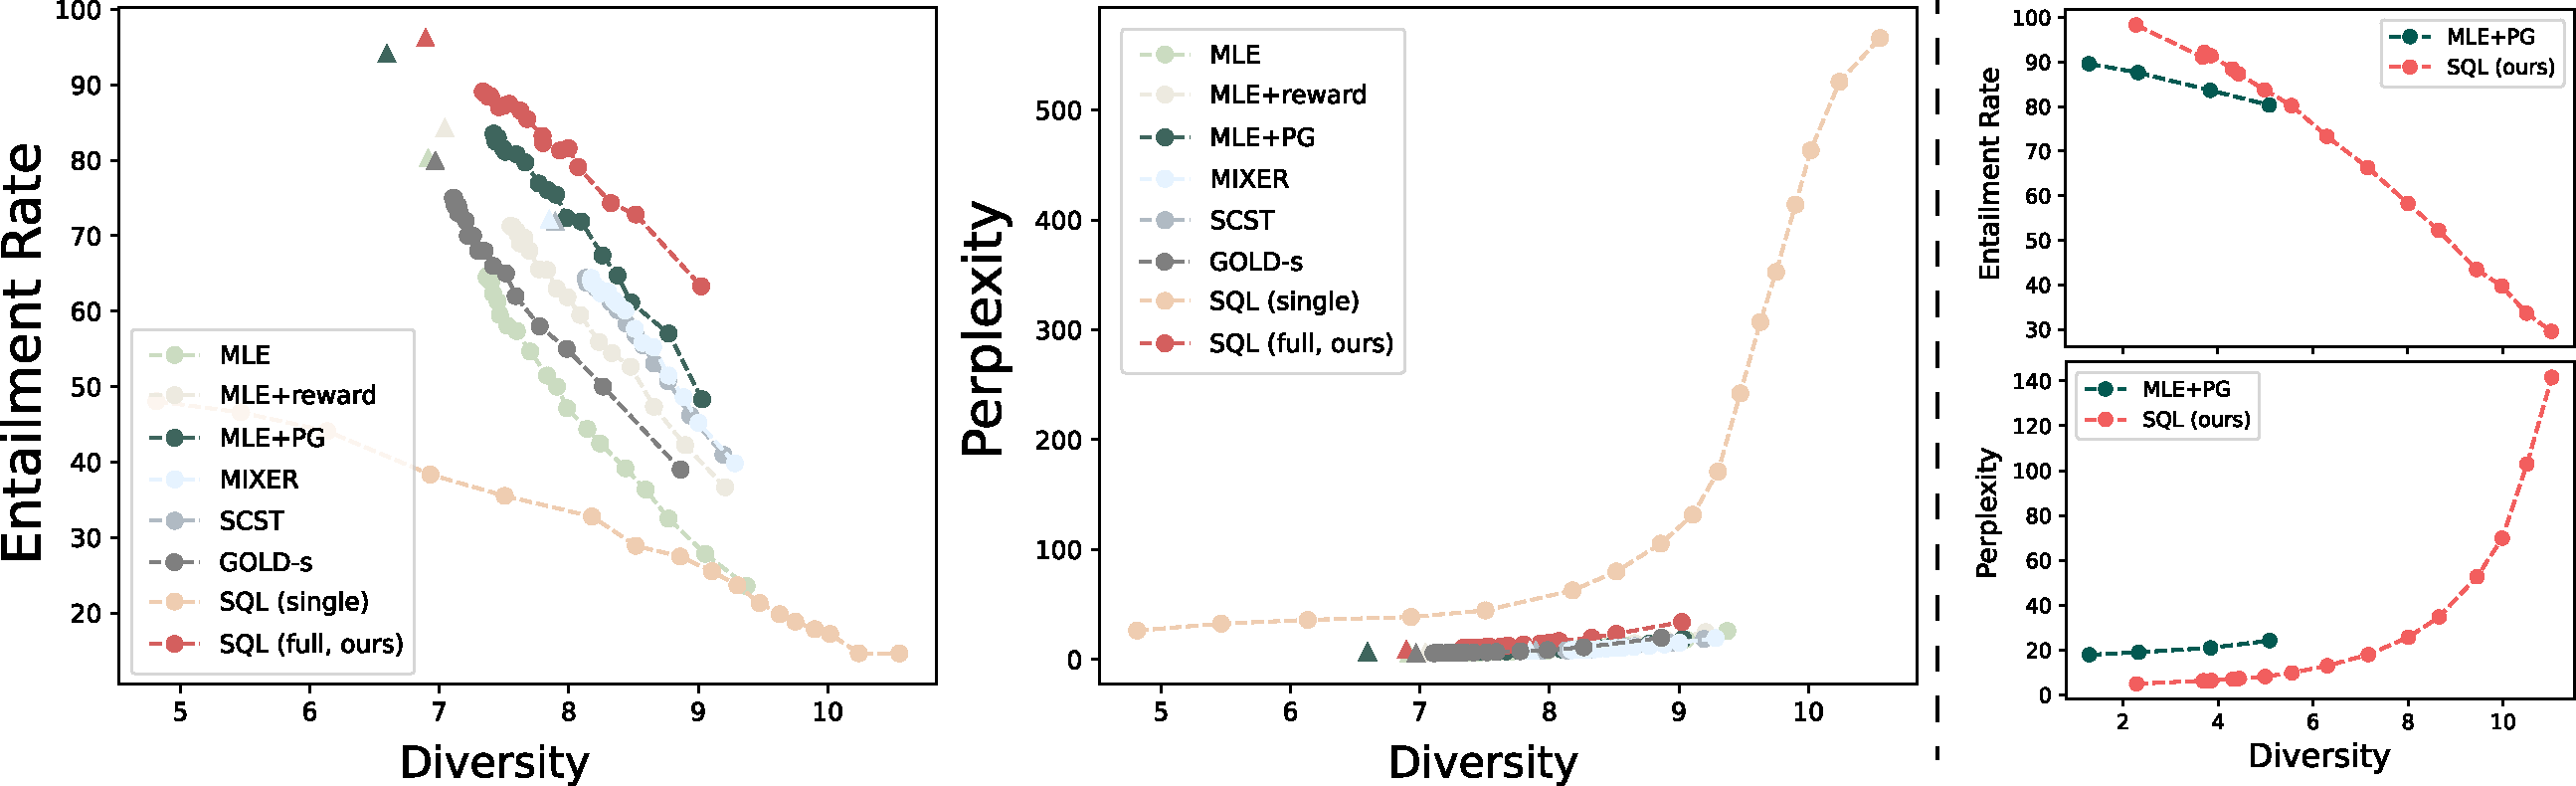
\includegraphics[width=0.99\linewidth]{figures/202101005-entailment-combined.pdf}
    \vspace{-7pt}
    \caption{
    \textbf{Left:} entailment generation performance plotted against diversity (average of $H_1$ and $H_2$). 
    Circles represent results of top-$p$ sample outputs,
    and triangles represent results of beam-search outputs.
    Please see Table~\ref{table:entailment-generation} for additional results.
    \textbf{Right:} entailment attack performance against diversity. 
    Only a few \texttt{MLE+PG} dots are visible because the model is not able to generate more diverse samples even with increasing $p$ value in top-$p$ decoding, i.e., the model collapses.
    }
    \label{fig:entailment-generation}
    \label{fig:entailment-attack}
    \vspace{-5pt}
\end{figure*}


\paragraph{Setup (more in~\S\ref{appendix-subsubsec:setup-noisy-data}).}
We sub-sampled $50k$ training examples from the SNLI dataset~\citep{bowman2015large}, a commonly used entailment classification dataset. The hypotheses have an average entailment probability of only $50\%$, and over $2/5$ of them less than $20\%$ (negative/contradictive examples) -- a significant challenge for the models to learn from the noises. 
The rewards include (1) the entailment score of the generation measured by a robust entailment classifier~\citep{nie2020adversarial}, (2) the log-likelihood of the generation as an indicator of language quality measured by a GPT-2 language model~\citep{radford2019language}, and (3) BLEU score w.r.t the input premises as another language quality reward that avoids trivial outputs. We sum together all rewards with weights $1.0$.

We compare our approach with a broad range of baselines, including 
(1) the standard MLE training (\texttt{MLE}); 
(2) \texttt{MLE+reward}, where we use the reward function to filter examples;
(3) joint MLE and PG training with MLE initialization (\texttt{MLE+PG}), where we initialize the model with MLE training, then train it with combined MLE and PG losses;
previous text-generation RL algorithms including (4) \texttt{MIXER}~\citep{ranzato2015sequence}, 
(5) \texttt{Self-critic}~\citep{rennie2017self}, 
and 
(6) one of the latest methods \texttt{GOLD-$s$}~\citep{pang2021text} which is a pure off-policy method based on importance-sampling PG. 
To ablate the effect of multi-step training (\S\ref{subsec:method:pcl}), we additionally compare with a simplified variant of our approach that uses only vanilla single-step PCL training (\texttt{SQL(single)}). We include more baselines such as MLE weighted by rewards in \S\ref{appendix-subsubsec:experiments-noisy-data}.




We evaluate generation results in terms of entailment rate, language quality (perplexity), and diversity which is measured by the Shannon entropy over unigrams and bigrams ($H_1$, $H_2$) \citep{gehrmann2021gem}. Since text generation models intrinsically
trade off diversity and quality \citep{caccia2019language,hashimoto2019unifying}, we vary the generation diversity by generating samples via top-$p$ sampling \citep{holtzman2019curious} with different $p$ values, and plot the entailment rate and perplexity against diversity, resp. We also evaluate the samples produced by beam-search decoding.

\paragraph{Results.}
Figure~\ref{fig:entailment-generation} (left) shows the results, and Table~\ref{table:entailment-generation-examples-sql} shows samples.
First, notice that \texttt{MLE} performs poorly, while \texttt{MLE+reward} improves upon it. This is not surprising as the training data contain noisy/negative examples. Similarly, since the pure off-policy algorithm \texttt{GOLD-$s$} relies heavily on the data distribution, we observed that it achieves sub-optimal performance. The on-policy \texttt{MLE+PG} with MLE initialization gives better entailment rate.
In comparison, our full \texttt{SQL} framework achieves the best entailment-diversity trade-off. 
The comparison between \texttt{SQL} and \texttt{SQL(single)} highlights the importance of having the multi-step objective which directly uses the end reward rather than bootstrapping intermediate $Q$-values for supervision.



















\subsection{\textit{Universal} Adversarial Attacks}
\label{subsec:adversarial-attack}

We next study the application
in text adversarial attacks, where again no supervised data is available. 
Adversarial attacks is an increasingly important research topic as they reveal models' vulnerabilities and flaws. This is especially true for universal attacks~\citep{wallace2019universal,atanasova2020generating}, where we want to generate universal examples that trick the model on \emph{all} possible inputs. 
For instance, consider the context of entailment classification.
Our goal is to find universal human-readable hypotheses that are going to be classified as ``entailment'' with as high probability as possible, regardless of the input premises. This is a more challenging setting compared to previous instance-specific attack \citep{morris2020textattack,jin2020bert,ebrahimi2017hotflip} where the attack model conditions on a premise and generates an adversarial hypothesis specific to the premise. 


\paragraph{Setup (more in~\S\ref{appendix-subsubsec:setup-adversarial-attack}).}
We aim to attack one of the most popular MultiNLI~\citep{williams2018broad} entailment classifiers on HuggingFaceHub.\footnote{\url{https://github.com/pytorch/fairseq/tree/master/examples/roberta}
} The attack generation model generates adversarial text without conditioning on any inputs so that the generated attacks are universal to all premises.  
We compare our \texttt{SQL} with \texttt{MLE+PG}. We use all hypotheses in the MultiNLI dataset as the training data for the MLE training in \texttt{MLE+PG} and the off-policy updates for our \texttt{SQL}.
We do not compare with previous specialized adversarial text attack methods, because they either are not applicable to the challenging universal attack setting \citep{morris2020textattack,jin2020bert,ebrahimi2017hotflip}, or were not designed to generate human-readable sentences \citep{wallace2019universal}. 
We use similar settings as in \S\ref{subsec:noisy-data} to explore the diversity-quality trade-off 
by plotting the entailment rate and perplexity against diversity, respectively. 
The entailment classifier to be attacked is used as entailment score reward functions. We also include a token-level repetition penalty reward for readability.


\paragraph{Results.}

Figure~\ref{fig:entailment-attack} (right) shows the results, and Table~\ref{table:entailment-attack-examples} shows samples.
We can see that \texttt{SQL} outperforms \texttt{MLE+PG} consistently across different diversity values. The outputs from \texttt{MLE+PG} are not diverse even with high $p$'s, indicating the model collapses and can only generate a small set of unique adversarial examples. 
The model by \texttt{SQL} discovers the pattern ``saint-pierre-et-saint-paul'' (an entity name), and exploits this to generate samples with high universal entailment rate.


\begin{figure}[t]
    \centering
    \begin{minipage}{.49\textwidth}
        \centering
        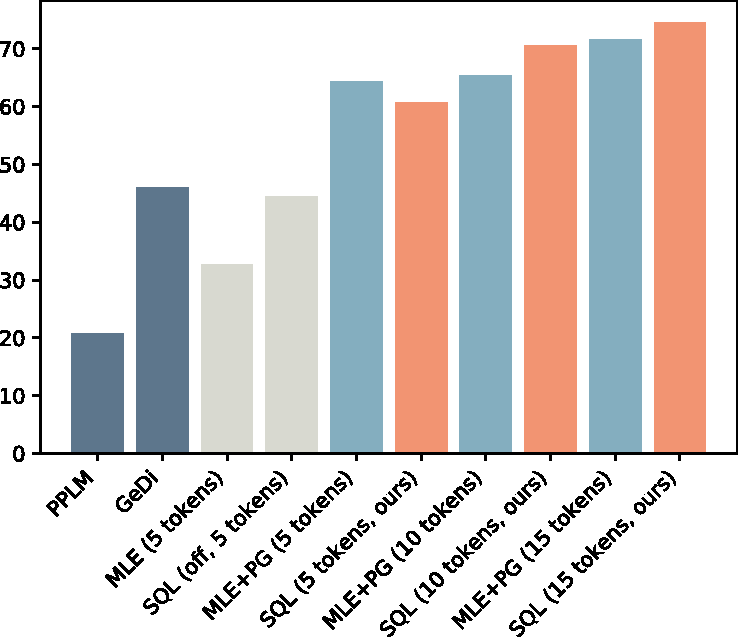
\includegraphics[width=0.75\linewidth]{figures/20210527.prompt-generation.pdf}
        \vspace{-7pt}
        \caption{Average topic accuracy. Please see Table~\ref{table:prompt-generation-full} for more details.}
        \label{fig:prompt-generation-topic}
\end{minipage}%
\hfill
\begin{minipage}{0.49\textwidth}
\centering
\small
\begin{tabular}{@{}llll@{}}
\toprule
\textbf{PPLM} & \textbf{GeDi} & \textbf{MLE (5)} & \textbf{SQL (off, 5)} \\
\midrule
$13.07$ & $123.88$ & $25.70$ & $25.77$ \\
\midrule
\multicolumn{2}{l}{\textbf{MLE+PG (5/10/15)}} & \multicolumn{2}{l}{\textbf{SQL (5/10/15, ours)}} \\
\midrule
\multicolumn{2}{l}{$25.52$/$28.16$/$28.71$} & \multicolumn{2}{l}{$25.94$/$26.95$/$29.10$} \\
\bottomrule
\end{tabular}
\vspace{-7pt}
\captionof{table}{
Average perplexity across topics. The lower, the more fluent the generated continuation sentences.
}
\vspace{-5pt}
\label{table:prompt-generation}

\vspace{9pt}

\centering
\small
\begin{tabular}{p{0.79cm}p{0.6cm}p{0.6cm}p{0.6cm}}
\toprule
\textbf{Model} & PPLM & GeDi & SQL \\
\midrule
\textbf{Seconds} & $5.58$ & $1.05$ & $0.07$ \\
\bottomrule
\end{tabular}
\vspace{-7pt}
\caption{Average sentence generation time cost.}
\vspace{-7pt}
\label{table:prompt-generation-speed}
\end{minipage}
\vspace{-7pt}
\end{figure}


\subsection{Prompt Generation for Controlling Pretrained Language Models}
\label{subsec:prompt-generation}





A reward function does not just have to be a metric like the BLEU score, but also a complicated pipeline that eventually returns a score.
To demonstrate this, we consider the emerging task of prompting a large pretrained LM for controllable generation \citep{Hu2017TowardCG,radford2019language,NEURIPS2020_1457c0d6}.
The goal is to learn to generate text prompts that steer the LM to generate sentences of certain desired attributes (e.g., topics). 
The problem of controlling the generation of pretrained LMs was previously approached through specialized algorithms such as modifying the LM hidden states during decoding~\citep{Dathathri2020Plug,krause2020gedi,qin2020backpropagation}. Here we show that prompts offer an easier, faster, more effective way for controlled generation.

Learning to generate/tune prompts is gaining increasing attention recently.
It side-steps the needs for expensive LM fine-tuning, and adapts LMs to new scenarios with prompt as the (compute-friendly) interface.
Most existing approaches~\citep{wallace2019universal,li2021prefix,lester2021power} rely on gradient backpropagation and are applicable only when the whole training pipeline is differentiable.
This does not hold for the text generation setting, as illustrated in Figure~\ref{fig:prompt-generation-flow}. In contrast, the RL framework is generally applicable to any differentiable or discrete pipelines.


\begin{figure}
\centering
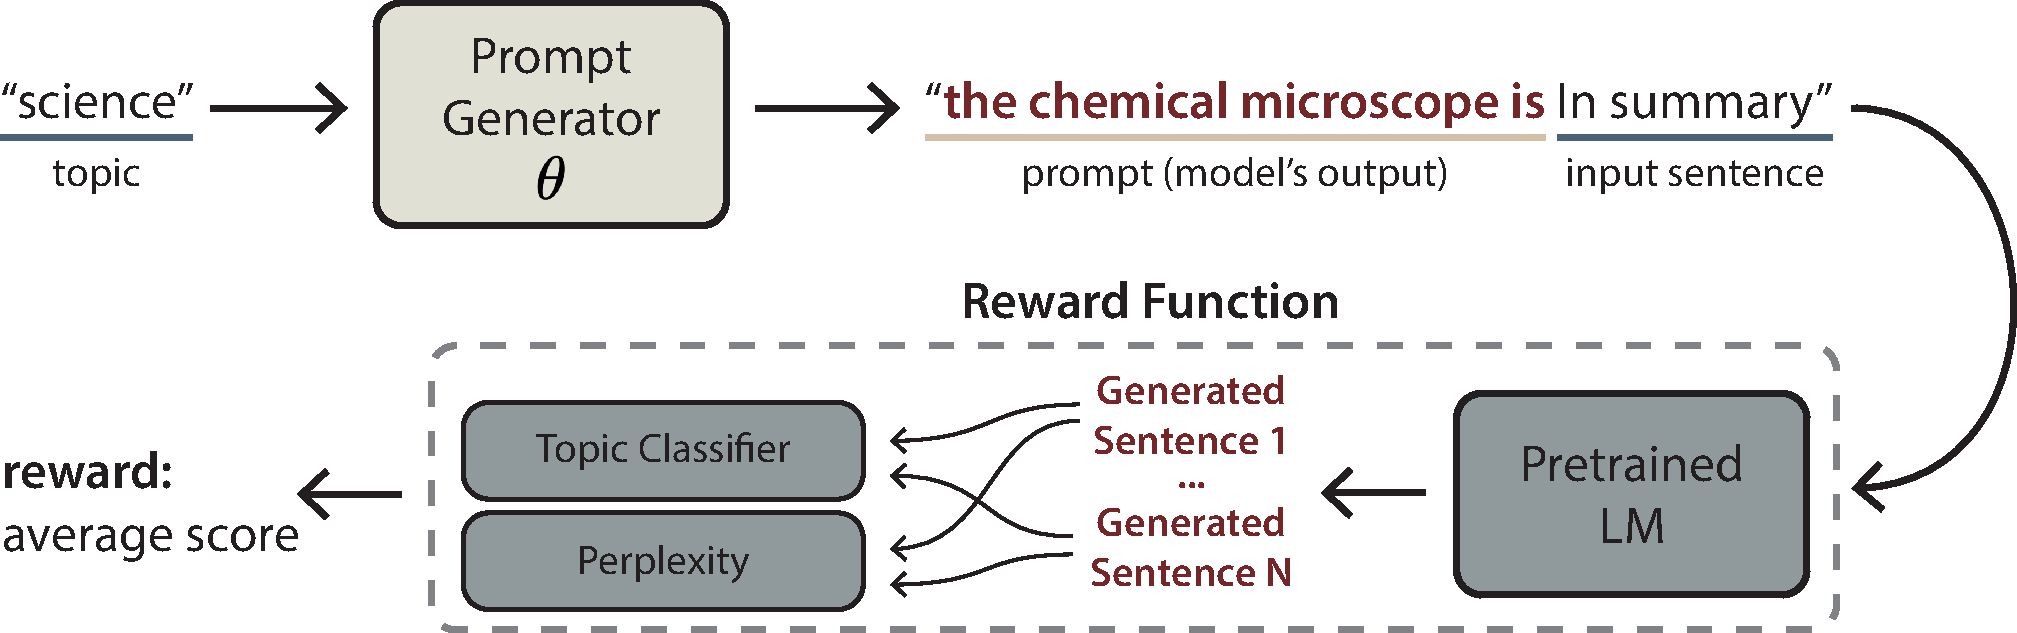
\includegraphics[width=0.99\linewidth]{figures/prompt-generation-task-new.pdf}
\vspace{-12pt}
\caption{
The scheme of prompt generation for controlling the outputs of pretraind LMs.
}
\vspace{-7pt}
\label{fig:prompt-generation-flow}
\end{figure}


\paragraph{Setup (more in~\S\ref{appendix-subsubsec:setup-prompt-generation}).}
Following \citep{dathathri2019plug}, we aim to control the generation to have one of 7 topics (e.g., ``science''); the generated prompt is prepended to one of 20 input sentences for the pretrained LM to generate continuation sentences. Figure~\ref{fig:prompt-generation-flow} shows the architecture of prompt-based controllable generation. We compare our \texttt{SQL} method with \texttt{MLE+PG} as before. Since the prompt length could impact the generated sentences, we conducted experiments with maximum prompt length $5$, $10$, and $15$. As ablation study, we also evaluate the SQL algorithm with only off-policy updates (i.e., without on-policy exploration), denoted as \texttt{SQL(off)}, and compare it with vanilla \texttt{MLE} training. Finally, we also compare with two specialized controllable generation techniques based on pretrained LMs, namely \texttt{PPLM}~\citep{dathathri2019plug} and \texttt{GeDi}~\citep{krause2020gedi}, following similar procedures using their open-sourced code. We use a distilled GPT-2 model\footnote{\url{https://huggingface.co/distilgpt2}} as the pretrained LM to be controlled. %
For rewards, we use the topic accuracy of the continuation sentences measured by a \emph{zero-shot} classifier, plus the the log-likelihood of continuation sentences as the language quality reward measured by a distilled GPT-2.\footnote{Note that the language quality emphasis is on the generated sentences. Prompts themselves do not necessarily have to be human-readable~\cite{wallace2019universal,sheng2020towards}.}


\paragraph{Results.}

Figure~\ref{fig:prompt-generation-topic} shows the topic accuracy of the controlled LM outputs averaged across the 7 topics, and Table~\ref{table:prompt-generation} shows the respective language quality results. More detailed topic accuracy results and samples are provided in the appendix (\S\ref{appendix-subsubsec:experiments-prompt-generation}) (where \texttt{GeDi} obtained low accuracy on 2 of the 7 topics, possibly because the topic tokens are tokenized into two subwords for which the model released by the authors was not specifically trained). 
We can see that the prompts generated by our \texttt{SQL} cause the LM to generate sentences with high topic accuracy while maintaining low perplexity in most settings.
Increasing the prompt length positively impacts the topic accuracy, which makes sense because longer prompts give more flexible for steering the LM.
The comparison between \texttt{MLE} and \texttt{SQL(off)}
shows that the off-policy component of SQL is better than standard MLE training, as it incorporates reward signals instead of just blindly following the (noisy) data. 

Next, comparing with the previous steered decoding such as \texttt{PPLM} and \texttt{GeDi},
we can see the prompt-based control trained with RL achieves better trade-off between topic accuracy and language quality. Moreover, once a prompt is produced, we can use the pretrained LM to generate text of desired topics efficiently, with the same time cost as standard non-controlled decoding. In comparison, the dedicated steered decoding is often orders-of-magnitude slower, as shown in Table~\ref{table:prompt-generation-speed}.






\section{Related Work}


\subsection{Overestimation in Reinforcement Learning}


The problem of overestimation in Q-learning with function approximation was introduced by \cite{Thrun+Schwartz:1993}.
For discrete actions the double estimator has been proposed \cite{hasselt2010double} where two Q-functions are learned and one is used to determine the maximizing action, while the other evaluates the Q-function for that action. The Double DQN algorithm extended this to neural networks~\cite{hasselt2016deepdouble}.
However, Zhang \emph{et al.} \cite{weightedQlearning} observed that the double estimator sometimes underestimates the Q-value and propose to use a weighted average of the single and the double estimator as target. This work is similar to ours in the regard that depending on the parameter over- or underestimation could be corrected. A major difference to our algorithm is that the weighting parameter is computed from the maximum and minimum of the estimated Q-value and does not use unbiased rollouts.
Similarly, the weighted estimator
\cite{cini2020deep,d2017estimating} 
estimates the maximum over actions in the TD target as the sum of values weighted by their probability of being the maximum. In continuous action spaces this can be done through Gaussian process regression
\cite{d2017estimating} and for discrete actions via dropout variational inference \cite{cini2020deep}.
Different to ACC the weighting is computed from the same off-policy data used to compute the single quantities while ACC adjusts the weighting parameter $\beta$ in a separate process using the latest on-policy rollouts.
Lv \emph{et al.} \cite{lvSDDQ19} use a similar weighting but suggest a stochastic selection of either the single or double estimator. The probability of choosing one or the other follows a predefined schedule.
Other approaches compute the weighted average of the minimum and maximum over different Q-value estimates \cite{fujimoto2019off,kumarStabilizing19}. However, the weighting parameter is a fixed hyperparameter.
The TD3 algorithm~\cite{td3} uses the minimum over two Q-value estimates as TD target. 
Maxmin Q-learning is another approach for discrete action spaces using an ensemble of Q-functions. For the TD target, first  the minimum of over all Q-functions is computed followed by maximization with respect to the action~\cite{Lan2020Maxmin}. Decreasing the ensemble size increases the estimated targets while increasing the size decreases the targets. Similarly to TQC this provides a way to control the bias in a more fine-grained way; the respective hyperparameter has to be set before the start of the training for each environment, however.
Cetin \emph{et al.}  \cite{cetin2021learning} propose to learn a pessimistic penalty to overcome the overestimation bias.

What sets ACC apart from the previously mentioned works is that unbiased on-policy rollouts are used to adjust a term that controls the bias correction instead of using some predefined heuristic. 






\subsection{Combining On- and Off-Policy Learning}
There are many approaches that combine on- and off-policy learning by combining policy gradients with off-policy samples
\cite{degris2012off,NIPS2010_35cf8659,o2016combining}.
In \cite{NIPS2017_IPG} an actor-critic is used where the critic is updated off-policy and the actor is updated with a mixture of policy gradient and Q-gradient. This differs from our work in that we are interested only in better critic estimates through the information of on-policy samples. 
To learn better value estimates by combining on- and off-policy data prior works proposed the use of some form of importance sampling
\cite{NIPS2014_be53ee61,precup2000eligibility}.
In \cite{hausknecht2016policy} the TD target is computed by mixing Monte Carlo samples with the bootstrap estimator.
These methods provide a tradeoff between variance and bias. They differ from our work in using the actual returns directly in the TD targets while we incorporate the returns indirectly via another parameter.
Bhatt \emph{et al.} \cite{bhatt2019crossnorm} propose the use of a mixture of on- and off-policy transitions to generate a feature normalization that can be used in off-policy TD learning. Applied to TD3, learning becomes more stable eliminating the need to use a delayed target network.



\subsection{Hyperparameter Tuning for Reinforcement Learning}

Most algorithms that tune hyperparameters of RL algorithms use many different instances of the environment to find a good setting
\cite{chiang19,falkner18a,jaderberg2017population}. 
There is, however, also work that adjusts a hyperparameter online during training \cite{xu2018meta}. In this work the meta-gradient (i.e., the gradient of the update rule) is used to adjust the discount factor and the length of bootstrapping intervals. However, it would not be straightforward to apply this method to control the bias of the value estimate. Their method also differs from ours in that they do not use a combination of on- and off-policy data.





\section{Conclusion}
We develop a new RL formulation for text generation based on soft $Q$-learning and path consistency learning.
We conduct experiments on learning with noisy and negative data, black box adversarial attack, prompting a pretrained language model for controllable generation, and  standard supervised tasks. This formulation opens up new opportunities to integrate more advances made in the fertile RL literature to improve text
generation problems. 




% \clearpage

% \appendix
% % \onecolumn
\section{Proof of Theorem 1}

% The estimator  $\qhatpi_{\beta^*}\sa$ was defined via
% \begin{equation}
%     \beta^* \sa = \argmin_{\beta \in [\bmin, \bmin]} \Bigg| \qhat_\beta \sa - \frac{1}{N} \sum_{i=1}^{N} R_i \sa  \Bigg| .
% \end{equation}

% To declutter the notation we drop the dependencies on the state-action pairs $\sa$ and the policy $\pi$.
Let $\Bar{R} = \frac{1}{N} \sum_{i=1}^{N} R_i $.
First note that the average of symmetrically distributed random variables is still a symmetric distributed random variable and hence 
$\Bar{R} $ is symmetrically distributed.
By assumption $\qhat_{\bmin}$ and $\qhat_{\bmax}$ have the same  distance to the true Q-value which is the mean $Q=\E[\Bar{R}] $, i.e. there is a real value $d$ such that
$Q = \qhat_{\bmin} +d = \qhat_{\bmax} -d$
denote the tail probability  P($\Bar{R} < \qhat_{\bmin}) = p_t$.  
Because of the symmetry and the same distance to the mean we also have that  $P(\Bar{R} > \qhat_{\bmax}) = p_t$.
% In the computation of $\E [ \qhat_{\beta^*} ]$  we can differentiate three events.
% If $\qhat_{\bmin} \leq \Bar{R} \leq \qhat_{\bmax}$ then $\qhat_{\beta^*} =\Bar{R}$, 
% if $\qhat_{\bmin} \geq \Bar{R}$ then $\qhat_{\beta^*} =\qhat_{\bmin}$
% and if $\qhat_{\bmin} \geq \Bar{R}$ then $\qhat_{\beta^*} =\qhat_{\bmax}$.
% We denote the indicator function with $\idc{A}$, which is equal to $1$ if the event $A$ is true and $0$ otherwise.
Then we get
\vspace{-0.1cm}
\begin{align*}
   &\E \big[ \qhat_{\beta^*} \big] 
   = \E \big[ \idc{\qhat_{\bmin} \leq \Bar{R} \leq \qhat_{\bmax}} \Bar{R}  \big]  \\
  & ~+  \E \big[ \idc{\qhat_{\bmin} \geq \Bar{R} }  \qhat_{\bmin} \big] +  \E \big[ \idc{\qhat_{\bmax} \leq \Bar{R} }  \qhat_{\bmax} \big]  \\
    &= (1-2p_t) \cdot \E[\Bar{R}] + p_t \E\big[\qhat_{\bmin}\big] + p_t \E\big[\qhat_{\bmax}\big] \\
   &= (1-2p_t) Q + p_t \qhat_{\bmin}+ p_t \qhat_{\bmax}\\
   &= (1-2p_t) Q + p_t (Q-d) + p_t (Q+d) = Q.
%   &= (1-2p_t) Q + 2p_t Q + p_t(d-d) \\
%   & = Q
\end{align*}




%  long proof

% The estimator  $\qhatpi_{\beta^*}\sa$ was defined via
% \begin{equation}
%     \beta^* \sa = \argmin_{\beta \in [\bmin, \bmin]} \Bigg| \qhat_\beta \sa - \frac{1}{N} \sum_{i=1}^{N} R_i \sa  \Bigg| .
% \end{equation}

% To declutter the notation we drop the dependencies on the state-action pairs $\sa$ and the policy $\pi$.
% Further we write $\Bar{R} = \frac{1}{N} \sum_{i=1}^{N} R_i $.
% First note that the average of symmetrically distributed random variables is still a symmetric distributed random variable and hence 
% $\Bar{R} $ is symmetrically distributed.
% By assumption $\qhat_{\bmin}$ and $\qhat_{\bmax}$ have the same  distance to the true Q-value which is the mean $Q=\E[\Bar{R}] $, i.e. there is a real value $d$ such that
% $Q = \qhat_{\bmin} +d = \qhat_{\bmax} -d$
% denote the tail probability  P($\Bar{R} < \qhat_{\bmin}) = p_t$.  Because of the symmetry and the same distance to the mean we also have that  $P(\Bar{R} > \qhat_{\bmax}) = p_t$.
% In the computation of $\E [ \qhat_{\beta^*} ]$  we can differentiate three events.
% If $\qhat_{\bmin} \leq \Bar{R} \leq \qhat_{\bmax}$ then $\qhat_{\beta^*} =\Bar{R}$, 
% if $\qhat_{\bmin} \geq \Bar{R}$ then $\qhat_{\beta^*} =\qhat_{\bmin}$
% and if $\qhat_{\bmin} \geq \Bar{R}$ then $\qhat_{\beta^*} =\qhat_{\bmax}$.
% We denote the indicator function with $\idc{A}$, which is equal to $1$ if the event $A$ is true and $0$ otherwise.
% Then we get

 
% \begin{align*}
%   \E \Big[ \qhat_{\beta^*} \Big] 
% %   &= \E \Bigg[ \min_{\beta \in [\bmin, \bmin]} \Big| \qhat_\beta  - \Bar{R}   \Big| \Bigg] \\
% %   &=  \E \Bigg[ \idc{\qhat_{\bmin} \leq \Bar{R} \leq \qhat_{\bmax}} 
% %   \min_{\beta \in [\bmin, \bmin]} \Big| \qhat_\beta  - \Bar{R}  \Big| \Bigg]  \\
% %   &~~~~+  \E \Bigg[ \idc{\qhat_{\bmin} \geq \Bar{R} }
% %   \min_{\beta \in [\bmin, \bmin]} \Big| \qhat_\beta  - \Bar{R}  \Big| \Bigg] \\
% %   &~~~~+ \E \Bigg[ \idc{\qhat_{\bmax} \leq \Bar{R} }
% %   \min_{\beta \in [\bmin, \bmin]} \Big| \qhat_\beta  - \Bar{R}  \Big| \Bigg] \\
%   &= \E \Bigg[ \idc{\qhat_{\bmin} \leq \Bar{R} \leq \qhat_{\bmax}} \Bar{R}  \Bigg]  \\
%   &~~~~+  \E \Bigg[ \idc{\qhat_{\bmin} \geq \Bar{R} }  \qhat_{\bmin} \Bigg] \\
%   &~~~~+  \E \Bigg[ \idc{\qhat_{\bmax} \leq \Bar{R} }  \qhat_{\bmax}  \Big| \Bigg]  \\
% %   +  \E \Bigg[ \idc{\qhat_{\bmin} \geq \Bar{R} }  \qhat_{\bmin} \Bigg] 
% %   +  \E \Bigg[ \idc{\qhat_{\bmax} \leq \Bar{R} }  \qhat_{\bmax}  \Big| \Bigg]  \\
%   &= (1-2p_t) \cdot \E[\Bar{R}] + p_t \E\Big[\qhat_{\bmin}\Big] + p_t \E\Big[\qhat_{\bmax}\Big] \\
%   &= (1-2p_t) Q + p_t \qhat_{\bmin}+ p_t \qhat_{\bmax}\\
%   &= (1-2p_t) Q + p_t (Q-d) + p_t (Q+d)\\
%   &= (1-2p_t) Q + 2p_t Q + p_t(d-d) \\
%   &= Q
% \end{align*}











% \section{Using Fewer Critic Networks for Faster Runtime}
% \label{app:2_nets}

% \begin{figure*}[b]
% \centering
% \begin{subfigure}{0.48\textwidth}
%   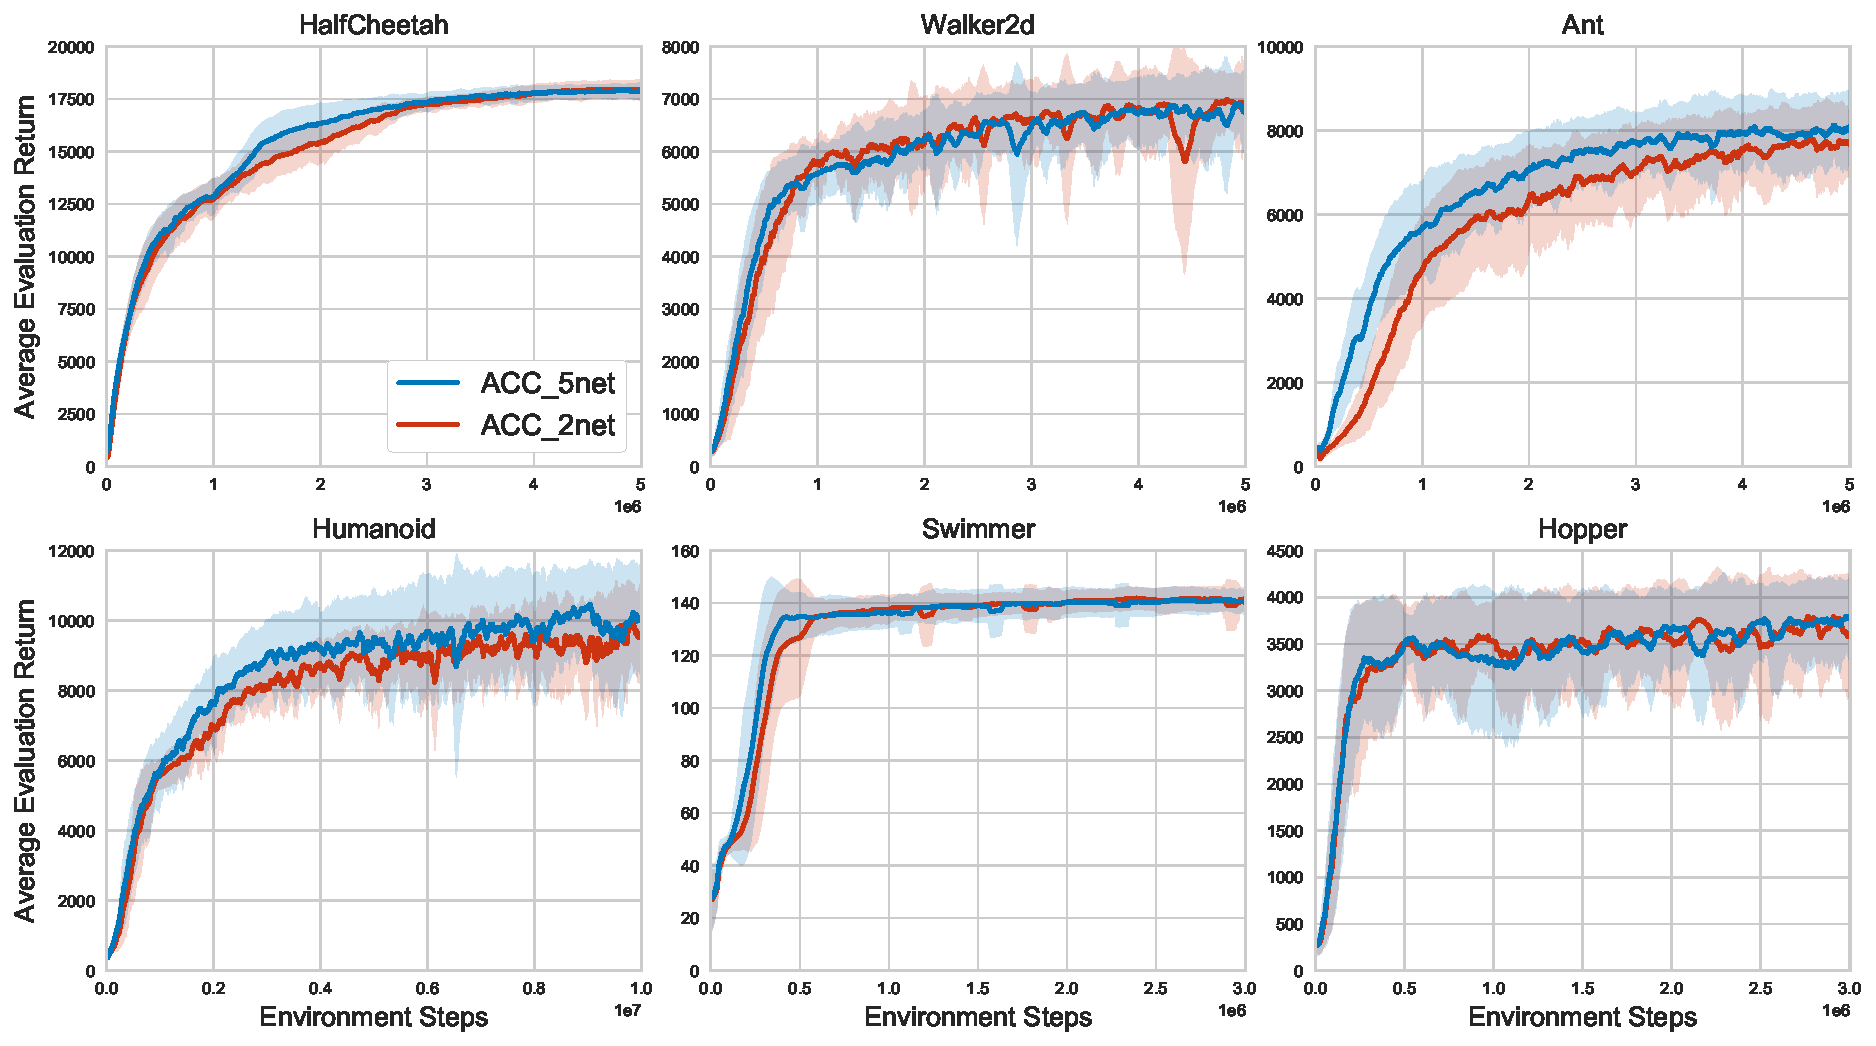
\includegraphics[width=1\linewidth]{images/ablation/2net_one_fig.pdf}
% \end{subfigure}
% \caption{The mean $\pm$ standard deviation over $10$ trials. 
% Results with different choices for the number of critic networks for each algorithm. }
% \label{fig:num_critic_nets}
% \end{figure*}
% Using $5$ critic networks - the default in TQC - to approximate the value function leads to a high runtime of the algorithm. It is possible to trade off performance against runtime by changing the number of critic networks. We evaluated ACC applied to TQC with $2$ networks and compare it to the standard setting with $5$ networks in Figure \ref{fig:num_critic_nets}. The results show that reducing the number of critic networks to $2$ leads only to a small drop in performance while the runtime is more than $2$ times faster.


% \section{Pseudocode}
% \label{app:pseudocode}


% \begin{algorithm}[t]
%   \caption{ACC - General}
%   \label{alg:general_acc}
% \begin{algorithmic}
%   \STATE {\bfseries Initialize:} bias controlling parameter $\beta$, steps between $\beta$ updates $T_\beta$, $t_\beta = 0$
%   \FOR{$t=1$ {\bfseries to} total number of environment steps}
%   \STATE Interact with environment according to $\pi$, store transitions in replay buffer $\mathcal{B}$ and store observed returns $R\sa$, increment $t_\beta \pluseq 1$
%   \IF{episode ended \textbf{and} $t_\beta >= T_\beta$}
%   \STATE Update $\beta$ with Eq. \ref{eq:one_step_beta_update} using the most recent experience and set $t_\beta=0$
%   \ENDIF
% %   \FOR{$j=1$ {\bfseries to} number Q-updates per environment step}
%   \STATE Sample mini-batch $b$ from $\mathcal{B}$
%   \STATE Update $Q$ with target computed from $\qbeta$ and $b$
% %   \ENDFOR
%   \ENDFOR
% \end{algorithmic}
% \end{algorithm}


% In Algorithm \ref{alg:general_acc} the general version of ACC is presented.
% The pseudocode for ACC applied to TQC is in Algorithm \ref{alg:acc_applied_to_tqc}.
% As the number of dropped targets per network is given by $d= d_{\max} - \beta $, we state the pseudocode in terms of the parameter $d$ instead of $\beta$. 


% \begin{algorithm}[t]
%   \caption{ACC - Applied to TQC}
%   \label{alg:acc_applied_to_tqc}
% \begin{algorithmic}
%   \STATE {\bfseries Initialize:} $d$ the bias controlling parameter, $\alpha$ the learning rate for $d$, $T_d$ the minimum number of steps between updates to $d$, $T_d^{init}$  the initial steps before $d$ is updated,
%   $S_R$ the size from which on episodes are removed from the batch storing the most recent returns, moving average parameter $\tau_d$, $t_d = 0$
%   \FOR{$t=1$ {\bfseries to} total number of environment steps}
%   \STATE Interact with environment according to $\pi$, store transitions in replay buffer $\mathcal{B}$ and, increment $t_d \pluseq 1$
%     \IF{episode ended}
%   \STATE Store observed returns $R\sa$ and corresponding state-action pairs $\sa$ in $\mathcal{B}_R$

   
%   \IF{ $t_d >= T_d$ \textbf{and} $t > T_d^{init}$}
%   \STATE $C = \sum_{ (s,a, R) \in \mathcal{B}_R} \Big[   Q \sa - R \sa  \Big]$,     $ma = (1-\tau_d) ma + \tau_d C$
%   \STATE $d = d + \alpha \frac{C}{ma}$, clip $d$ in interval $[0, d_{max}]$, set $t_d=0$
%     \STATE Remove the oldest episodes from $\mathcal{B}_R$ until there are at most $S_R$ left
%   \ENDIF
%   \ENDIF
% %   \FOR{$j=1$ {\bfseries to} number Q-updates per environment step}
%   \STATE Sample mini-batch from $\mathcal{B}$
%   \STATE Update critic $Q$ as in TQC, where $dN$ (rounded to the next integer) number of targets are dropped from the set of pooled targets 
%   \STATE Update policy $\pi$ as in TQC 
% %   \ENDFOR
%   \ENDFOR
% \end{algorithmic}
% \end{algorithm}


 








% \section{Hyperparameters}
% \label{app:hyperparameter}

% At the beginning of the training we initialize $\beta = 2.5$ and set the step size parameter to $\alpha=0.1$.
% After $T_\beta = 1000$ steps since the last update and when the next episode finishes, $\beta$ is updated with a batch that stores the most recent state-action pairs encountered in the environment and their corresponding observed discounted returns. 
% The choice of $T_\beta$ was motivated by the fact that the maximum duration of an episode is $1000$ steps for the considered environments.
% After every update of $\beta$ the oldest episodes in this stored batch are removed until there are no more than $5000$ state-action pairs left. This means that on average $\beta$ is updated with a batch whose size is a bit over $5000$. 
% The updates of $\beta$ are started as soon as $25000$ environment steps as completed and
% the moving average parameter in the normalization of the $\beta-$update is set to $0.05$. 
% The  first $5000$ environment interactions are generated with a random policy after which learning starts.
% Apart from that all hyperparameters are the same as in TQC with $N=5$ critic networks.
% In Table \ref{tab:hyperparameter} we list all hyperparameters of ACC applied to TQC.

% In the following we also desribe the process of hyperparameter selection.
% The range of values $d$ is allowed to take is set to the interval $[0,5]$ as it includes the optimal hyperparameters for TQC from all environments, which are in the set $\{0,2,5\}$. We did not try higher values than $5$.
% The initial value for number of dropped targets per network was set to $2.5$ as this value is in the middle of the allowed range and did not evaluated other choices.
% The learning rate $\alpha$ of $d$ was set to $0.1$ based on visual inspection of how fast $d$ changes. We  evaluated $\alpha=0.05$ for a small subset of tasks and seeds, but $\alpha=0.1$ gave slightly better results.
% $T_d$ was set to $1000$ as the episode length is $1000$ and we did not evaluate other choices.
% For $T_d^{init}$ we evaluated the choices $10000$ and $25000$ on a small subset of environments and seeds and did not found a big impact on performance. As $d$ changes very quickly in the beginning we chose $T_d^{init}=25000$.
% For $S_R$ we evaluated the choices $1000$ and $5000$ also on a small subset of environments and seeds and found $5000$ to perform slightly better.
% We did not tune the moving average parameter and set it to $\tau_d = 0.05$.
% For all hyperparameters for which we evaluated more than one choice we do not have definite results as the number of seeds and environments were limited.
% The hyperparameters shared with TQC were not changed.




% \begin{table}[h]
% \caption{Hyperparameters values.}
% \label{tab:hyperparameter}
% \vskip 0.15in
% \begin{center}
% \begin{small}
% \begin{sc}
% \begin{tabular}{lccc}
% \toprule
% Hyperparameter & \multicolumn{3}{c}{ACC} \\
% \midrule
% Optimizer & \multicolumn{3}{c}{Adam} \\
% Learning rate & \multicolumn{3}{c}{\num{3e-4}} \\
% Discount $\gamma$ & \multicolumn{3}{c}{0.99} \\
% Replay buffer size & \multicolumn{3}{c}{\num{1e6}} \\
% Number of critics $N$ & \multicolumn{3}{c}{5} \\
% Number of atoms $M$ & \multicolumn{3}{c}{25}\\
% Huber loss parameter  & \multicolumn{3}{c}{1} \\
% Number of hidden layers in critic networks & \multicolumn{3}{c}{3}\\
% Size of hidden layers in critic networks & \multicolumn{3}{c}{512} \\
% Number of hidden layers in policy network & \multicolumn{3}{c}{2} \\
% Size of hidden layers in policy network & \multicolumn{3}{c}{256} \\
% Minibatch size & \multicolumn{3}{c}{256} \\
% Entropy target  &  \multicolumn{3}{c}{$- \dim \mathcal{A}$} \\
% Nonlinearity & \multicolumn{3}{c}{ReLU} \\
% Target smoothing coefficient  & \multicolumn{3}{c}{0.005} \\
% Target updates per critic gradient step & \multicolumn{3}{c}{1} \\
% Critic gradient steps per iteration & \multicolumn{3}{c}{1} \\
% Actor gradient steps per iteration & \multicolumn{3}{c}{1} \\
% Environment steps per iteration & \multicolumn{3}{c}{1} \\
% \midrule
% Initial value for number of dropped targets per network & \multicolumn{3}{c}{2.5} \\
% Maximum value for $d$ denoted $d_\max$ & \multicolumn{3}{c}{5} \\
% Minimum value for $d$ denoted $d_\min$ & \multicolumn{3}{c}{0} \\
% Learning rate for $d$ denoted $\alpha$ & \multicolumn{3}{c}{0.1} \\
% Minimum number of steps between updates to $d$ denoted $T_d$ & \multicolumn{3}{c}{1000} \\
% Initial number of steps before $d$ is updated denoted $T_d^{init}$ & \multicolumn{3}{c}{25000} \\
% Limiting size for batch used to update $d$ denoted $S_R$ & \multicolumn{3}{c}{5000} \\
% Moving average parameter $\tau_d$ & \multicolumn{3}{c}{0.05} \\
% \midrule
% \midrule
% Hyperparameter in Sample Efficient Experiment & ACC\_1q & ACC\_2q & ACC\_4q \\
% \midrule
% Critic gradient steps per iteration & 1 & 2 & 4 \\
% Actor gradient steps per iteration & 1 & 1 & 1 \\
% Target updates per critic gradient step & 1 & 1 & 1\\
% \bottomrule
% \end{tabular}
% \end{sc}
% \end{small}
% \end{center}
% \vskip -0.1in
% \end{table}




% $d$ the bias controlling parameter, $T_d$ the number of steps between updates to $d$, $T_d^{init}$  the initial steps before $d$ is updated,
%   $S_R$ the size from which on episodes are removed from the batch storing the most recent returns, moving average parameter $\tau_d$, $t_d = 0$


% \section{Potential Limitations}
% One limitation of our work is that ACC can not be applied in the offline RL setting, as ACC also uses on-policy data.
% Furthermore, in the stated form ACC relies on the episodic RL setting. However, we believe that ACC could potentially be adapted to that setting. 
% It is also not entirely clear how the algorithm would perform in the terminal reward setting, where a reward of for example $1$ is given upon successful completion of a specific task. While we do not have experiments for such environments we imagine that the positive effect of ACC could diminish as the true Q-values of states closer to the start of the episode are almost zero because of the discounting. 



% \section{Potential Negative Societal Impact}
% This work studied general and fundamental algorithms in the area of deep reinforcement learning. 
% Therefore, we do not see how this work could lead to a negative societal impact.



% \section{Analysis of the ACC Parameter}
% \label{app:analysis_acc_parameter}

% \begin{figure*}[b]
% \begin{subfigure}[b]{0.98\textwidth}
%   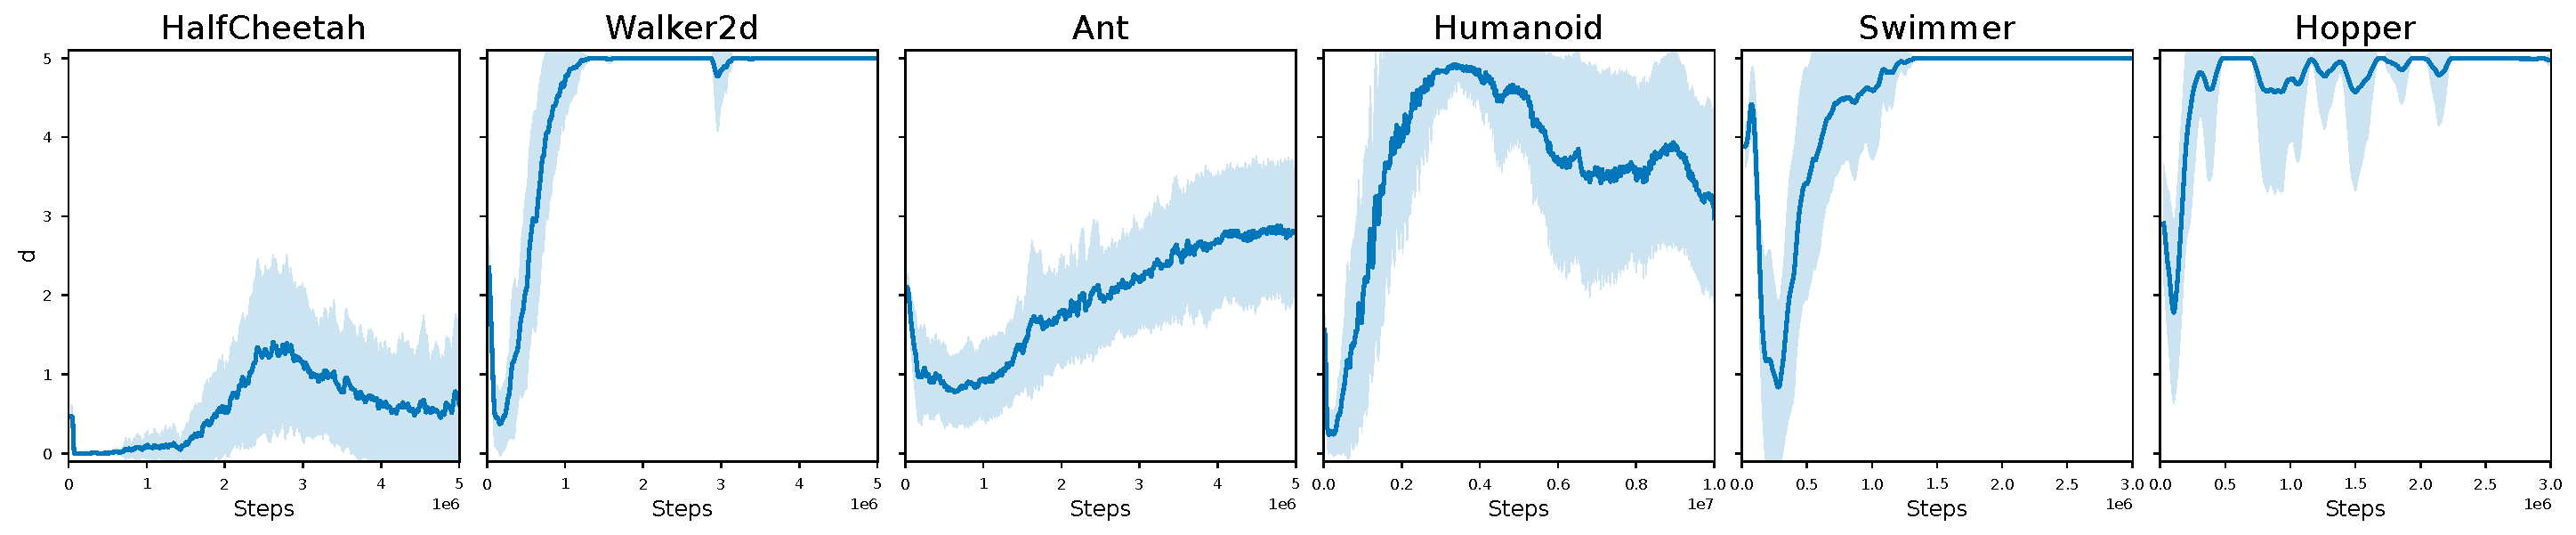
\includegraphics[width=1\linewidth]{images/analysis/visualize_beta_all_envs.pdf}
% \end{subfigure}
% \begin{subfigure}[b]{0.98\textwidth}
%   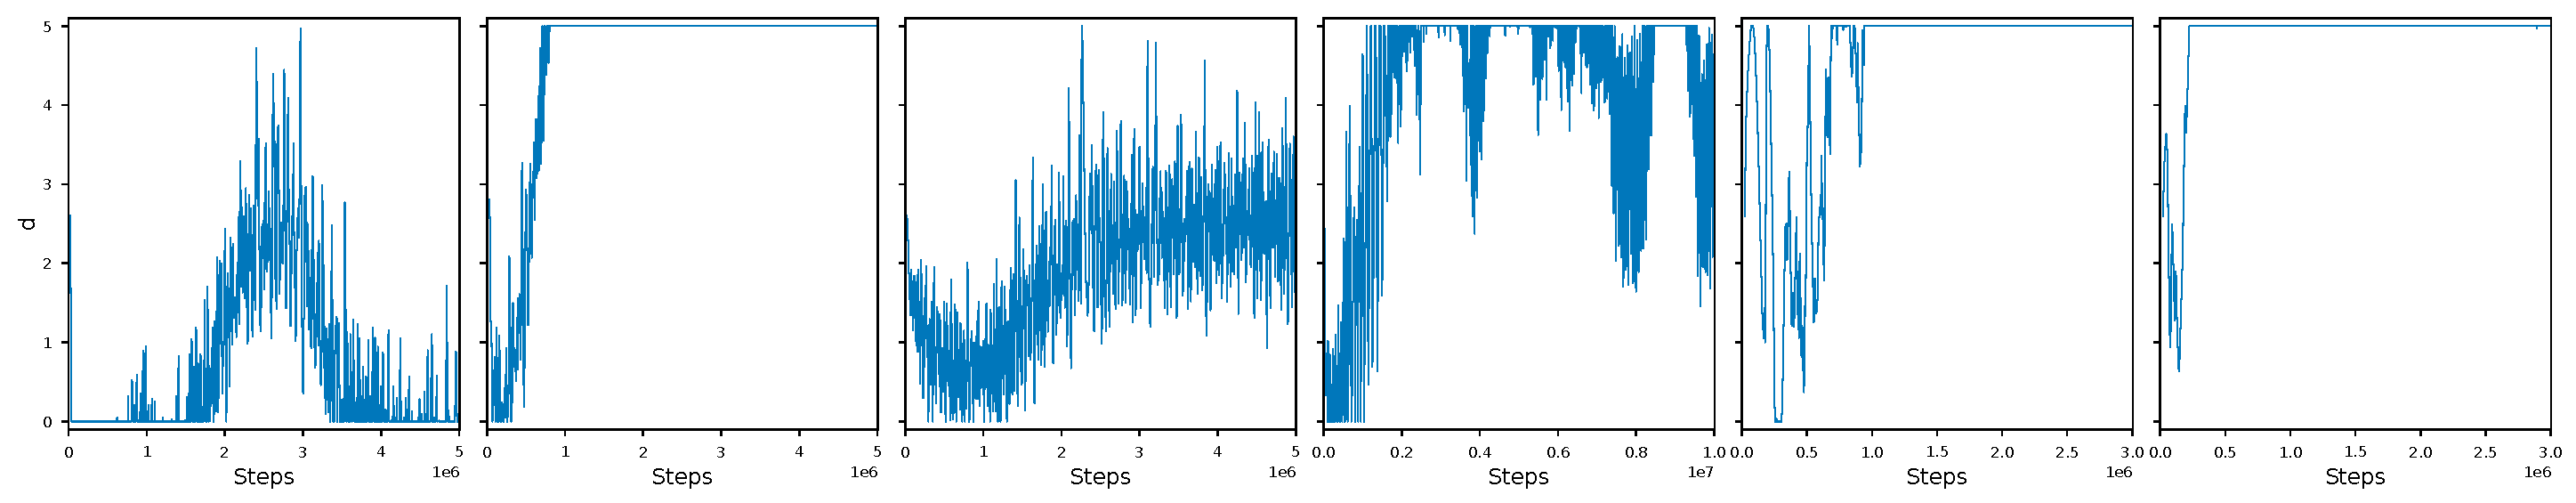
\includegraphics[width=1\linewidth]{images/analysis/visualize_beta_one_run_all_envs.pdf}
% \end{subfigure}

% \caption{Development of the number of dropped targets per network $d=d_{max}-\beta$ in ACC over time for different environments. The top row shows the mean (thick line) and standard deviation (shaded area) over the $10$ trials where for readability a uniform filter of size $15$ is used.
% The bottom row shows the unfiltered development for one of the seeds.}
% \label{fig:num_dropped_targets_all_envs}
% \end{figure*}

% % \begin{figure*}
% %     \centering
% %     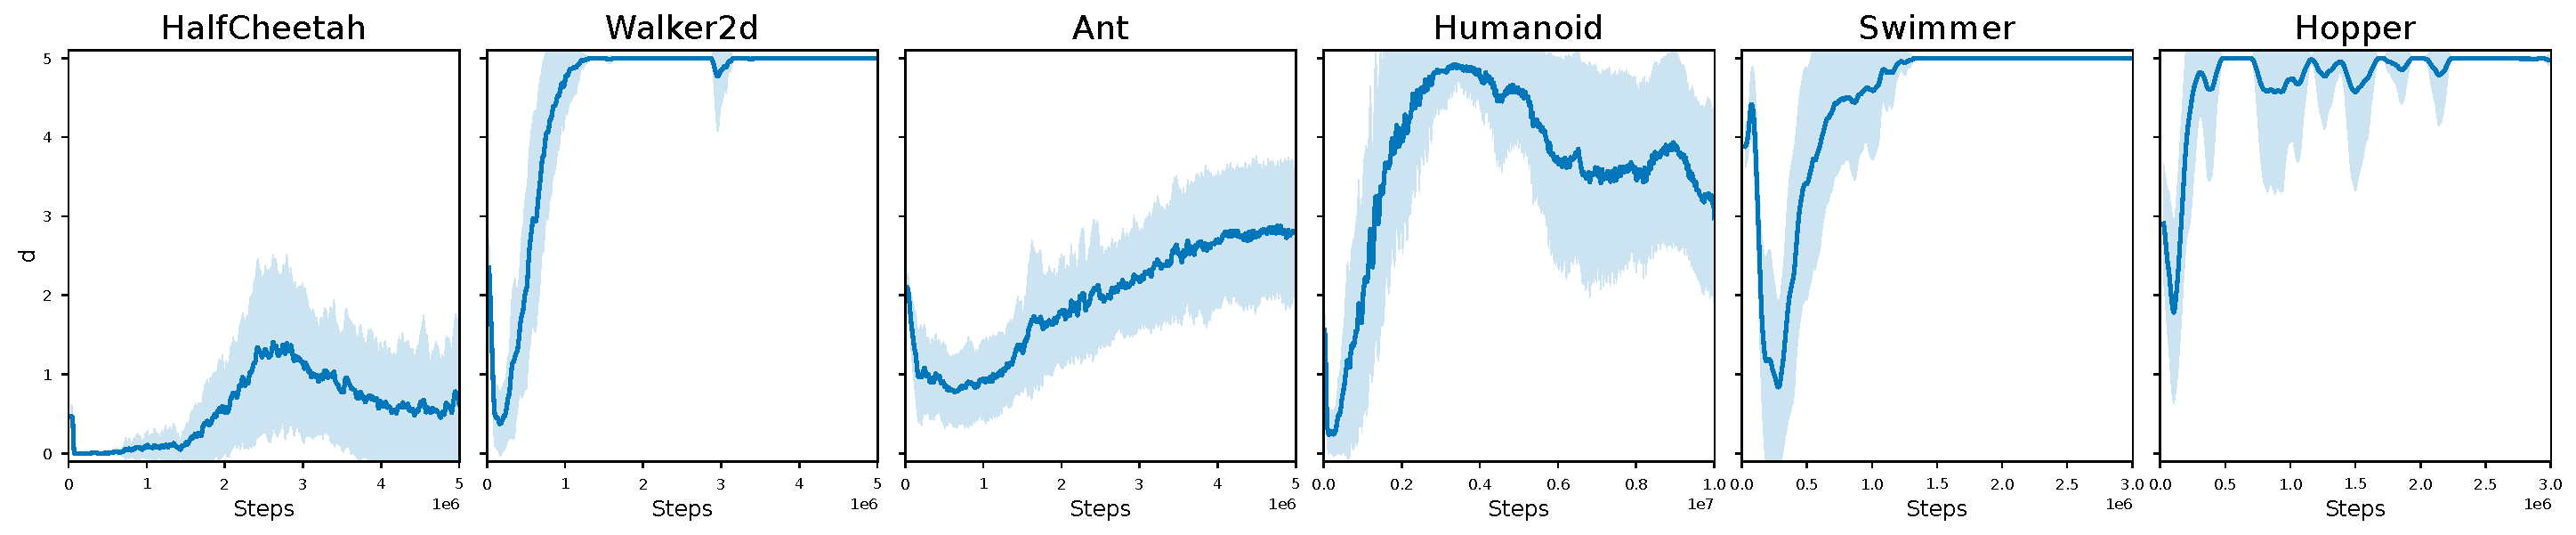
\includegraphics[width=0.98\textwidth]{images/analysis/visualize_beta_all_envs.pdf}
% %     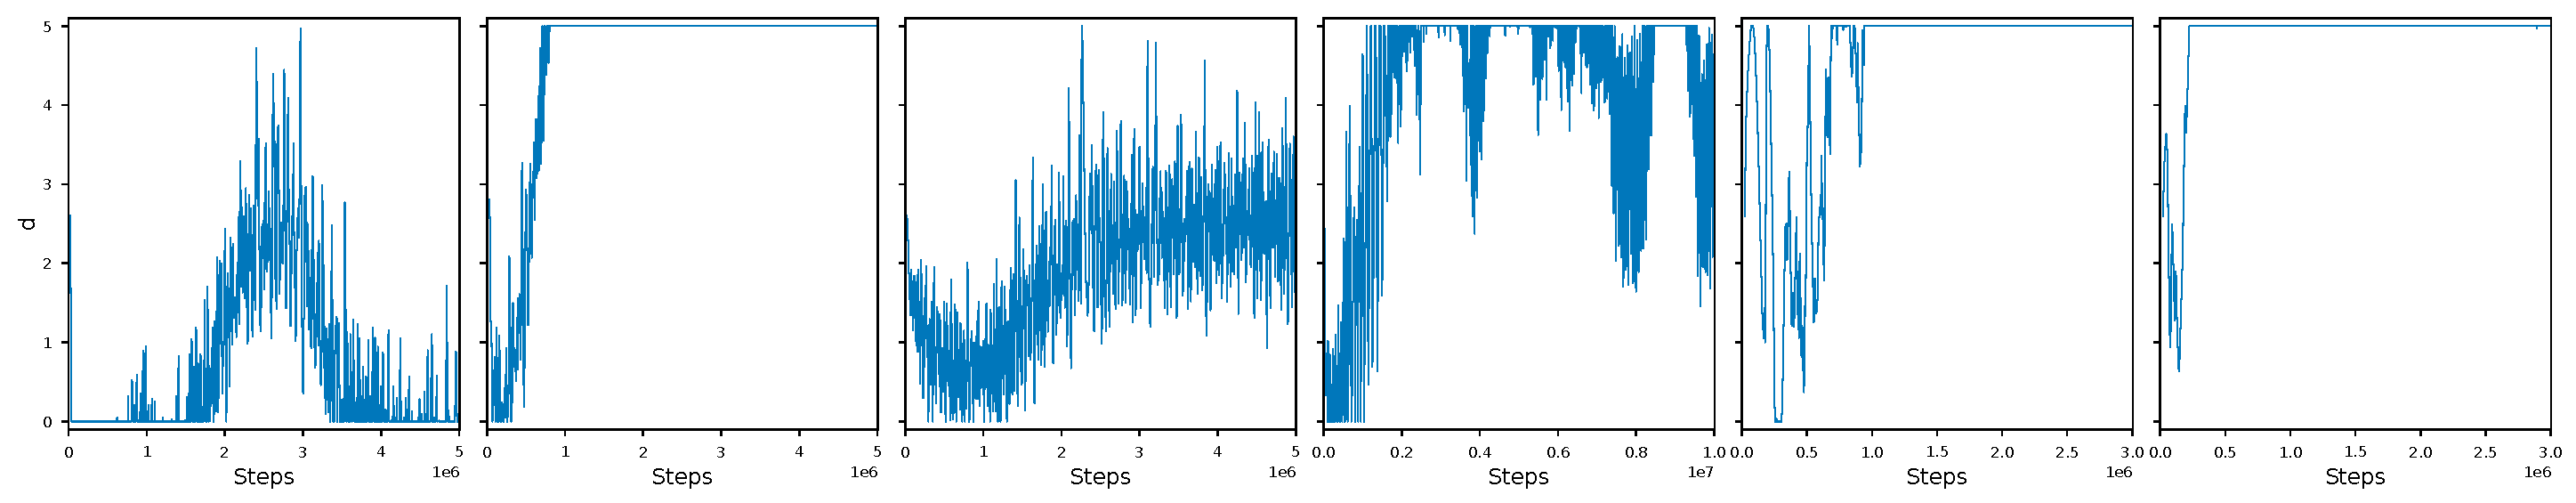
\includegraphics[width=0.98\textwidth]{images/analysis/visualize_beta_one_run_all_envs.pdf}
% %     \caption{Caption}
% %     \label{fig:my_label}
% % \end{figure*}



% To better understand the hidden training dynamics of ACC we show in 
% Figure \ref{fig:num_dropped_targets_all_envs}
% how the number of dropped targets per network $d=d_{max}-\beta$ evolves during training. 
% To do so we plotted $d$ after every $5000$ steps during the training of ACC.
% From the top row the first observation is that per environment the results are similar over the $10$ seeds as can be seen from the relatively low standard deviation. We show the single runs for all seeds in the appendix to further support this observation.
% However, there are large differences between the environments which supports the argument that it might not be possible to find a single hyperparameter that works well on a wide variety of different environments.
% Another point that becomes clear from the plots is that the optimal amount of overestimation correction might change over time during the training even on a single environment.

% In the bottom row of Figure \ref{fig:num_dropped_targets_all_envs} we plotted the evolution of $d$ for one of the $10$ trials in order to shed light on the actual training mechanics of a single run without lost information due to averaging.
% For each environment there is a trend but $d$ is also fluctuating to a certain degree.
% While this shows that the initial value of $d$ is not very important as the value quickly changes, this also highlights another interesting aspect of ACC. 
% The rollouts give highly fluctuating returns. The parameter $d=d_{max}-\beta$ is changing more slowly and picks up the trend. So a lot of the variance of the returns is filtered out in ACC by incorporating on-policy samples via the detour over $\beta$.
% This leads to relatively stable TD targets computed from $\qbeta$ while an upbuilding under- or overestimation is prevented as $\beta$ picks up the trend. On the other hand, if $\beta$ would change too slowly the upbuilding of the bias might not be stopped.








%\section*{ACKNOWLEDGMENT}
%Include already in submission?

\bibliographystyle{IEEEtran}
\bibliography{IEEEabrv,acc_bibliography}



% \onecolumn






\clearpage
% \appendix


\begin{strip}
\begin{center}
\vspace{-5ex}
\textbf{\LARGE \bf
Adaptively Calibrated Critic Estimates for \\ Deep Reinforcement Learning} \\
\vspace{2ex}

% \Large{\bf- Supplementary Material -}\\
\Large{\bf- Appendix -}\\
\vspace{0.4cm}
\normalsize{Nicolai Dorka\hspace{1cm} Tim Welschehold \hspace{1cm} Joschka Bödecker\hspace{1cm} Wolfram Burgard}\\
\end{center}
\end{strip}

\setcounter{section}{0}
\renewcommand{\thesection}{A.\arabic{section}}
\makeatletter

\section{Proof of Theorem 1}

The estimator  $\qhatpi_{\beta^*}\sa$ was defined via
\begin{equation}
    \beta^* \sa = \argmin_{\beta \in [\bmin, \bmin]} \Bigg| \qhat_\beta \sa - \frac{1}{N} \sum_{i=1}^{N} R_i \sa  \Bigg| .
\end{equation}

To declutter the notation we drop the dependencies on the state-action pairs $\sa$ and the policy $\pi$.
Further we write $\Bar{R} = \frac{1}{N} \sum_{i=1}^{N} R_i $.
First note that the average of symmetrically distributed random variables is still a symmetric distributed random variable and hence 
$\Bar{R} $ is symmetrically distributed.
By assumption $\qhat_{\bmin}$ and $\qhat_{\bmax}$ have the same  distance to the true Q-value which is the mean $Q=\E[\Bar{R}] $, i.e. there is a distance real valued value $d$ such that
$Q = \qhat_{\bmin} +d = \qhat_{\bmax} -d$
Denote the tail probabilty  P($\Bar{R} < \qhat_{\bmin}) = p_t$.  Because of the symmetry and the same distance to the mean we also have that  $P(\Bar{R} > \qhat_{\bmax}) = p_t$.
In the computation of $\E [ \qhat_{\beta^*} ]$  we can differentiate three events.
If $\qhat_{\bmin} \leq \Bar{R} \leq \qhat_{\bmax}$ then $\qhat_{\beta^*} =\Bar{R}$, 
if $\qhat_{\bmin} \geq \Bar{R}$ then $\qhat_{\beta^*} =\qhat_{\bmin}$
and if $\qhat_{\bmin} \geq \Bar{R}$ then $\qhat_{\beta^*} =\qhat_{\bmax}$.
We denote the indicator function with $\idc{A}$, which is equal to $1$ if the event $A$ is true and $0$ otherwise.
Then we get

 
\begin{align*}
   \E \Big[ \qhat_{\beta^*} \Big] 
%   &= \E \Bigg[ \min_{\beta \in [\bmin, \bmin]} \Big| \qhat_\beta  - \Bar{R}   \Big| \Bigg] \\
%   &=  \E \Bigg[ \idc{\qhat_{\bmin} \leq \Bar{R} \leq \qhat_{\bmax}} 
%   \min_{\beta \in [\bmin, \bmin]} \Big| \qhat_\beta  - \Bar{R}  \Big| \Bigg]  \\
%   &~~~~+  \E \Bigg[ \idc{\qhat_{\bmin} \geq \Bar{R} }
%   \min_{\beta \in [\bmin, \bmin]} \Big| \qhat_\beta  - \Bar{R}  \Big| \Bigg] \\
%   &~~~~+ \E \Bigg[ \idc{\qhat_{\bmax} \leq \Bar{R} }
%   \min_{\beta \in [\bmin, \bmin]} \Big| \qhat_\beta  - \Bar{R}  \Big| \Bigg] \\
   &= \E \Bigg[ \idc{\qhat_{\bmin} \leq \Bar{R} \leq \qhat_{\bmax}} \Bar{R}  \Bigg]  \\
  &~~~~+  \E \Bigg[ \idc{\qhat_{\bmin} \geq \Bar{R} }  \qhat_{\bmin} \Bigg] \\
  &~~~~+  \E \Bigg[ \idc{\qhat_{\bmax} \leq \Bar{R} }  \qhat_{\bmax}  \Big| \Bigg]  \\
%   +  \E \Bigg[ \idc{\qhat_{\bmin} \geq \Bar{R} }  \qhat_{\bmin} \Bigg] 
%   +  \E \Bigg[ \idc{\qhat_{\bmax} \leq \Bar{R} }  \qhat_{\bmax}  \Big| \Bigg]  \\
   &= (1-2p_t) \cdot \E[\Bar{R}] + p_t \E\Big[\qhat_{\bmin}\Big] + p_t \E\Big[\qhat_{\bmax}\Big] \\
   &= (1-2p_t) Q + p_t \qhat_{\bmin}+ p_t \qhat_{\bmax}\\
   &= (1-2p_t) Q + p_t (Q-d) + p_t (Q+d)\\
   &= (1-2p_t) Q + 2p_t Q + p_t(d-d) \\
   &= Q.
\end{align*}




\section{Pseudocode}
\label{app:pseudocode}


The pseudocode for ACC applied to TQC is in Algorithm \ref{alg:acc_applied_to_tqc}.
As the number of dropped targets per network is given by $d= d_{\max} - \beta $, we state the pseudocode in terms of the parameter $d$ instead of $\beta$. 


\begin{algorithm}[t]
   \caption{ACC - Applied to TQC}
   \label{alg:acc_applied_to_tqc}
\begin{algorithmic}
   \STATE {\bfseries Initialize:} $d$ the bias controlling parameter, $\alpha$ the learning rate for $d$, $T_d$ the minimum number of steps between updates to $d$, $T_d^{init}$  the initial steps before $d$ is updated,
   $S_R$ the size from which on episodes are removed from the batch storing the most recent returns, moving average parameter $\tau_d$, $t_d = 0$
   \FOR{$t=1$ {\bfseries to} total number of environment steps}
   \STATE Interact with environment according to $\pi$, store transitions in replay buffer $\mathcal{B}$ and, increment $t_d \pluseq 1$
    \IF{episode ended}
   \STATE Store observed returns $R\sa$ and corresponding state-action pairs $\sa$ in $\mathcal{B}_R$

   
   \IF{ $t_d >= T_d$ \textbf{and} $t > T_d^{init}$}
   \STATE $C = \sum_{ (s,a, R) \in \mathcal{B}_R} \Big[   Q \sa - R \sa  \Big]$,     $ma = (1-\tau_d) ma + \tau_d C$
   \STATE $d = d + \alpha \frac{C}{ma}$, clip $d$ in interval $[0, d_{max}]$, set $t_d=0$
    \STATE Remove the oldest episodes from $\mathcal{B}_R$ until there are at most $S_R$ left
   \ENDIF
   \ENDIF
%   \FOR{$j=1$ {\bfseries to} number Q-updates per environment step}
   \STATE Sample mini-batch from $\mathcal{B}$
   \STATE Update critic $Q$ as in TQC, where $dN$ (rounded to the next integer) number of targets are dropped from the set of pooled targets 
   \STATE Update policy $\pi$ as in TQC 
%   \ENDFOR
  \ENDFOR
\end{algorithmic}
\end{algorithm}


 


\section{Using Fewer Critic Networks for Faster Runtime}
\label{app:2_nets}

\begin{figure*}[t]
\centering
  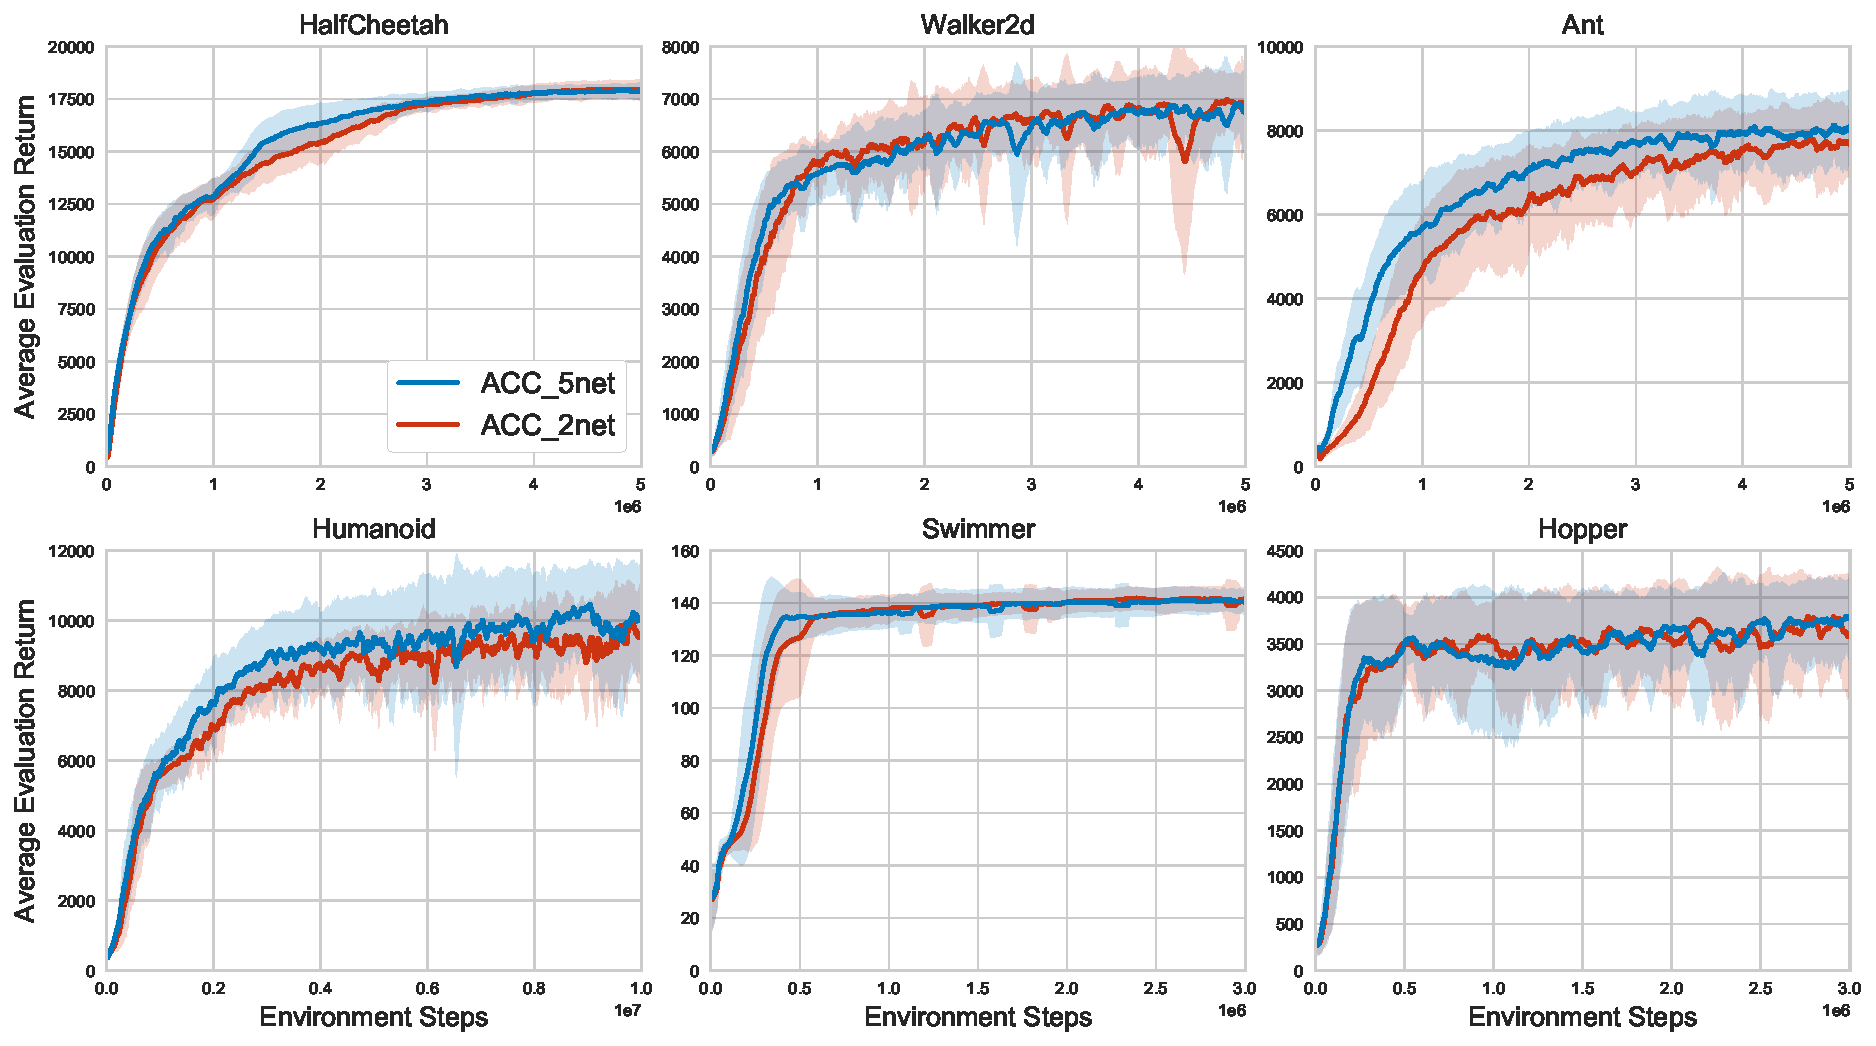
\includegraphics[width=.8\linewidth]{images/ablation/2net_one_fig.pdf}
\caption{The mean $\pm$ standard deviation over $10$ trials. 
Results with different choices for the number of critic networks for each algorithm. }
\label{fig:num_critic_nets}
\end{figure*}
Using $5$ critic networks - the default in TQC - to approximate the value function leads to a high runtime of the algorithm. It is possible to trade off performance against runtime by changing the number of critic networks. We evaluated ACC applied to TQC with $2$ networks and compare it to the standard setting with $5$ networks in Figure \ref{fig:num_critic_nets}. The results show that reducing the number of critic networks to $2$ leads only to a small drop in performance while the runtime is more than $2$ times faster.







\section{Hyperparameters}
\label{app:hyperparameter}

At the beginning of the training we initialize $\beta = 2.5$ and set the step size parameter to $\alpha=0.1$.
After $T_\beta = 1000$ steps since the last update and when the next episode finishes, $\beta$ is updated with a batch that stores the most recent state-action pairs encountered in the environment and their corresponding observed discounted returns. 
The choice of $T_\beta$ was motivated by the fact that the maximum duration of an episode is $1000$ steps for the considered environments.
After every update of $\beta$ the oldest episodes in this stored batch are removed until there are no more than $5000$ state-action pairs left. This means that on average $\beta$ is updated with a batch whose size is a bit over $5000$. 
The updates of $\beta$ are started as soon as $25000$ environment steps as completed and
the moving average parameter in the normalization of the $\beta-$update is set to $0.05$. 
The  first $5000$ environment interactions are generated with a random policy after which learning starts.
Apart from that all hyperparameters are the same as in TQC with $N=5$ critic networks.
In Table \ref{tab:hyperparameter} we list all hyperparameters of ACC applied to TQC.

In the following we also desribe the process of hyperparameter selection.
The range of values $d$ is allowed to take is set to the interval $[0,5]$ as it includes the optimal hyperparameters for TQC from all environments, which are in the set $\{0,2,5\}$. We did not try higher values than $5$.
The initial value for number of dropped targets per network was set to $2.5$ as this value is in the middle of the allowed range and did not evaluated other choices.
The learning rate $\alpha$ of $d$ was set to $0.1$ based on visual inspection of how fast $d$ changes. We  evaluated $\alpha=0.05$ for a small subset of tasks and seeds, but $\alpha=0.1$ gave slightly better results.
$T_d$ was set to $1000$ as the episode length is $1000$ and we did not evaluate other choices.
For $T_d^{init}$ we evaluated the choices $10000$ and $25000$ on a small subset of environments and seeds and did not found a big impact on performance. As $d$ changes very quickly in the beginning we chose $T_d^{init}=25000$.
For $S_R$ we evaluated the choices $1000$ and $5000$ also on a small subset of environments and seeds and found $5000$ to perform slightly better.
We did not tune the moving average parameter and set it to $\tau_d = 0.05$.
For all hyperparameters for which we evaluated more than one choice we do not have definite results as the number of seeds and environments were limited.
The hyperparameters shared with TQC were not changed.
For TD3 and SAC we used the hyperparameters from the respective papers.




\begin{table*}[t]
\caption{Hyperparameters values.}
\label{tab:hyperparameter}
\vskip 0.15in
\begin{center}
\begin{small}
\begin{sc}
\begin{tabular}{lccc}
\toprule
Hyperparameter & \multicolumn{3}{c}{ACC} \\
\midrule
Optimizer & \multicolumn{3}{c}{Adam} \\
Learning rate & \multicolumn{3}{c}{\num{3e-4}} \\
Discount $\gamma$ & \multicolumn{3}{c}{0.99} \\
Replay buffer size & \multicolumn{3}{c}{\num{1e6}} \\
Number of critics $N$ & \multicolumn{3}{c}{5} \\
Number of atoms $M$ & \multicolumn{3}{c}{25}\\
Huber loss parameter  & \multicolumn{3}{c}{1} \\
Number of hidden layers in critic networks & \multicolumn{3}{c}{3}\\
Size of hidden layers in critic networks & \multicolumn{3}{c}{512} \\
Number of hidden layers in policy network & \multicolumn{3}{c}{2} \\
Size of hidden layers in policy network & \multicolumn{3}{c}{256} \\
Minibatch size & \multicolumn{3}{c}{256} \\
Entropy target  &  \multicolumn{3}{c}{$- \dim \mathcal{A}$} \\
Nonlinearity & \multicolumn{3}{c}{ReLU} \\
Target smoothing coefficient  & \multicolumn{3}{c}{0.005} \\
Target updates per critic gradient step & \multicolumn{3}{c}{1} \\
Critic gradient steps per iteration & \multicolumn{3}{c}{1} \\
Actor gradient steps per iteration & \multicolumn{3}{c}{1} \\
Environment steps per iteration & \multicolumn{3}{c}{1} \\
\midrule
Initial value for number of dropped targets per network & \multicolumn{3}{c}{2.5} \\
Maximum value for $d$ denoted $d_{\max}$ & \multicolumn{3}{c}{5} \\
Minimum value for $d$ denoted $d_{\min}$ & \multicolumn{3}{c}{0} \\
Learning rate for $d$ denoted $\alpha$ & \multicolumn{3}{c}{0.1} \\
Minimum number of steps between updates to $d$ denoted $T_d$ & \multicolumn{3}{c}{1000} \\
Initial number of steps before $d$ is updated denoted $T_d^{init}$ & \multicolumn{3}{c}{25000} \\
Limiting size for batch used to update $d$ denoted $S_R$ & \multicolumn{3}{c}{5000} \\
Moving average parameter $\tau_d$ & \multicolumn{3}{c}{0.05} \\
\midrule
\midrule
Hyperparameter in Sample Efficient Experiment & ACC\_1q & ACC\_2q & ACC\_4q \\
\midrule
Critic gradient steps per iteration & 1 & 2 & 4 \\
Actor gradient steps per iteration & 1 & 1 & 1 \\
Target updates per critic gradient step & 1 & 1 & 1\\
\bottomrule
\end{tabular}
\end{sc}
\end{small}
\end{center}
\vskip -0.1in
\end{table*}






\section{Potential Limitations}
One limitation of our work is that ACC can not be applied in the offline RL setting, as ACC also uses on-policy data.
Furthermore, in the stated form ACC relies on the episodic RL setting. However, we believe that ACC could potentially be adapted to that setting. 
It is also not entirely clear how the algorithm would perform in the terminal reward setting, where a reward of for example $1$ is given upon successful completion of a specific task. While we do not have experiments for such environments we imagine that the positive effect of ACC could diminish as the true Q-values of states closer to the start of the episode are almost zero because of the discounting. 




\section{Analysis of the ACC Parameter}
\label{app:analysis_acc_parameter}

\begin{figure*}[b]
  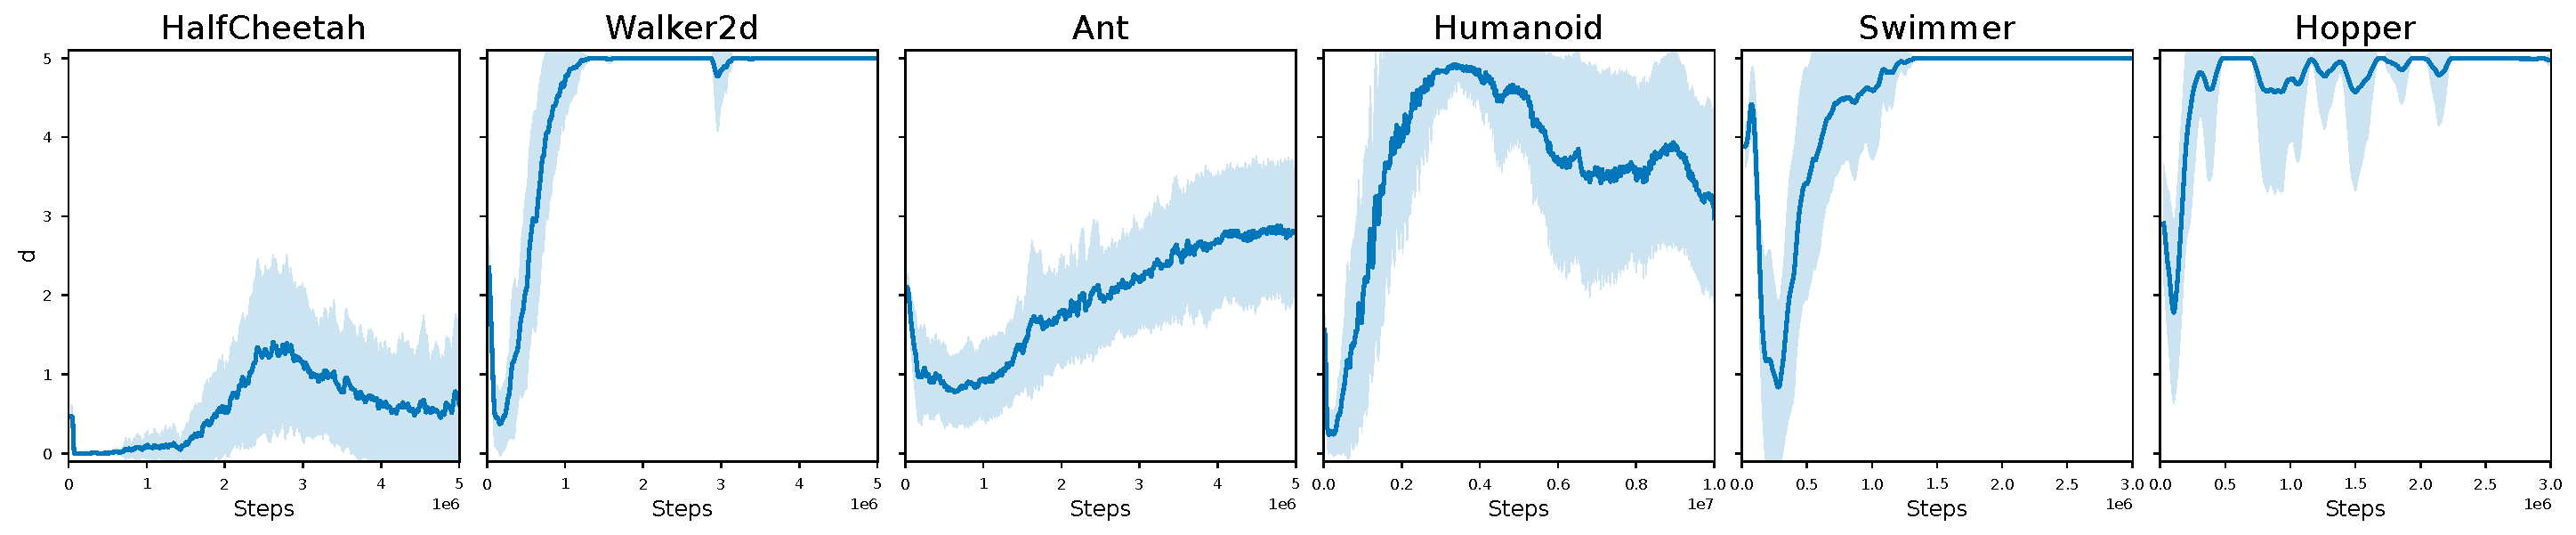
\includegraphics[width=1\linewidth]{images/analysis/visualize_beta_all_envs.pdf}
  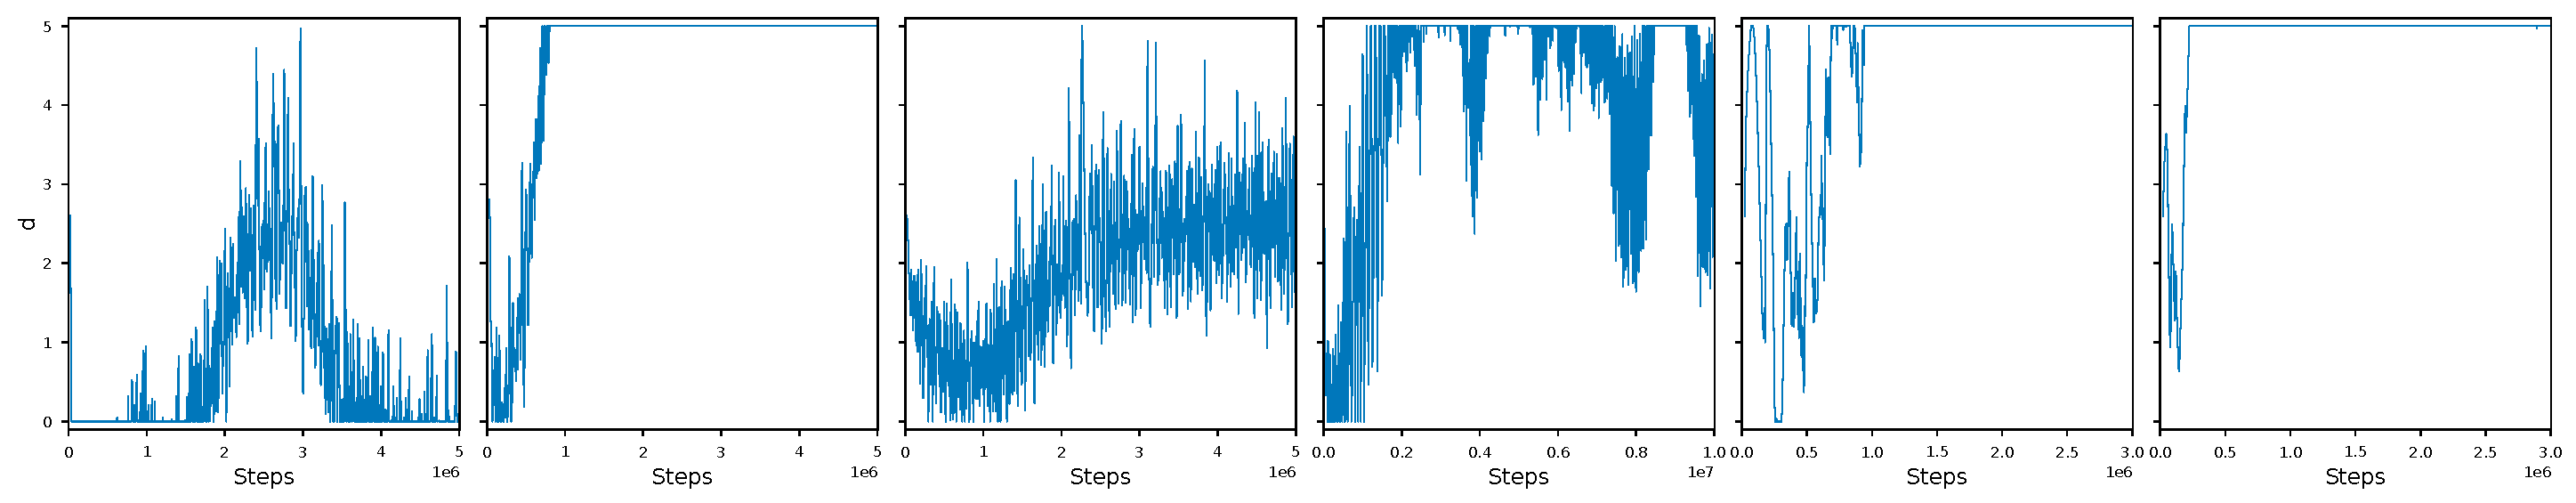
\includegraphics[width=1\linewidth]{images/analysis/visualize_beta_one_run_all_envs.pdf}
\caption{Development of the number of dropped targets per network $d=d_{max}-\beta$ in ACC over time for different environments. The top row shows the mean (thick line) and standard deviation (shaded area) over the $10$ trials where for readability a uniform filter of size $15$ is used.
The bottom row shows the unfiltered development for one of the seeds.}
\label{fig:num_dropped_targets_all_envs}
\end{figure*}




To better understand the hidden training dynamics of ACC we show in 
Figure \ref{fig:num_dropped_targets_all_envs}
how the number of dropped targets per network $d=d_{max}-\beta$ evolves during training. 
To do so we plotted $d$ after every $5000$ steps during the training of ACC.
From the top row the first observation is that per environment the results are similar over the $10$ seeds as can be seen from the relatively low standard deviation. We show the single runs for all seeds in the appendix to further support this observation.
However, there are large differences between the environments which supports the argument that it might not be possible to find a single hyperparameter that works well on a wide variety of different environments.
Another point that becomes clear from the plots is that the optimal amount of overestimation correction might change over time during the training even on a single environment.

In the bottom row of Figure \ref{fig:num_dropped_targets_all_envs} we plotted the evolution of $d$ for one of the $10$ trials in order to shed light on the actual training mechanics of a single run without lost information due to averaging.
For each environment there is a trend but $d$ is also fluctuating to a certain degree.
While this shows that the initial value of $d$ is not very important as the value quickly changes, this also highlights another interesting aspect of ACC. 
The rollouts give highly fluctuating returns. The parameter $d=d_{max}-\beta$ is changing more slowly and picks up the trend. So a lot of the variance of the returns is filtered out in ACC by incorporating on-policy samples via the detour over $\beta$.
This leads to relatively stable TD targets computed from $\qbeta$ while an upbuilding under- or overestimation is prevented as $\beta$ picks up the trend. On the other hand, if $\beta$ would change too slowly the upbuilding of the bias might not be stopped.

























% \addtolength{\textheight}{-12cm}   % This command serves to balance the column lengths
                                  % on the last page of the document manually. It shortens
                                  % the textheight of the last page by a suitable amount.
                                  % This command does not take effect until the next page
                                  % so it should come on the page before the last. Make
                                  % sure that you do not shorten the textheight too much.

%%%%%%%%%%%%%%%%%%%%%%%%%%%%%%%%%%%%%%%%%%%%%%%%%%%%%%%%%%%%%%%%%%%%%%%%%%%%%%%%



%%%%%%%%%%%%%%%%%%%%%%%%%%%%%%%%%%%%%%%%%%%%%%%%%%%%%%%%%%%%%%%%%%%%%%%%%%%%%%%%



%%%%%%%%%%%%%%%%%%%%%%%%%%%%%%%%%%%%%%%%%%%%%%%%%%%%%%%%%%%%%%%%%%%%%%%%%%%%%%%%





\end{document}
